\documentclass[1p]{elsarticle_modified}
%\bibliographystyle{elsarticle-num}

%\usepackage[colorlinks]{hyperref}
%\usepackage{abbrmath_seonhwa} %\Abb, \Ascr, \Acal ,\Abf, \Afrak
\usepackage{amsfonts}
\usepackage{amssymb}
\usepackage{amsmath}
\usepackage{amsthm}
\usepackage{scalefnt}
\usepackage{amsbsy}
\usepackage{kotex}
\usepackage{caption}
\usepackage{subfig}
\usepackage{color}
\usepackage{graphicx}
\usepackage{xcolor} %% white, black, red, green, blue, cyan, magenta, yellow
\usepackage{float}
\usepackage{setspace}
\usepackage{hyperref}

\usepackage{tikz}
\usetikzlibrary{arrows}

\usepackage{multirow}
\usepackage{array} % fixed length table
\usepackage{hhline}

%%%%%%%%%%%%%%%%%%%%%
\makeatletter
\renewcommand*\env@matrix[1][\arraystretch]{%
	\edef\arraystretch{#1}%
	\hskip -\arraycolsep
	\let\@ifnextchar\new@ifnextchar
	\array{*\c@MaxMatrixCols c}}
\makeatother %https://tex.stackexchange.com/questions/14071/how-can-i-increase-the-line-spacing-in-a-matrix
%%%%%%%%%%%%%%%

\usepackage[normalem]{ulem}

\newcommand{\msout}[1]{\ifmmode\text{\sout{\ensuremath{#1}}}\else\sout{#1}\fi}
%SOURCE: \msout is \stkout macro in https://tex.stackexchange.com/questions/20609/strikeout-in-math-mode

\newcommand{\cancel}[1]{
	\ifmmode
	{\color{red}\msout{#1}}
	\else
	{\color{red}\sout{#1}}
	\fi
}

\newcommand{\add}[1]{
	{\color{blue}\uwave{#1}}
}

\newcommand{\replace}[2]{
	\ifmmode
	{\color{red}\msout{#1}}{\color{blue}\uwave{#2}}
	\else
	{\color{red}\sout{#1}}{\color{blue}\uwave{#2}}
	\fi
}

\newcommand{\Sol}{\mathcal{S}} %segment
\newcommand{\D}{D} %diagram
\newcommand{\A}{\mathcal{A}} %arc


%%%%%%%%%%%%%%%%%%%%%%%%%%%%%5 test

\def\sl{\operatorname{\textup{SL}}(2,\Cbb)}
\def\psl{\operatorname{\textup{PSL}}(2,\Cbb)}
\def\quan{\mkern 1mu \triangleright \mkern 1mu}

\theoremstyle{definition}
\newtheorem{thm}{Theorem}[section]
\newtheorem{prop}[thm]{Proposition}
\newtheorem{lem}[thm]{Lemma}
\newtheorem{ques}[thm]{Question}
\newtheorem{cor}[thm]{Corollary}
\newtheorem{defn}[thm]{Definition}
\newtheorem{exam}[thm]{Example}
\newtheorem{rmk}[thm]{Remark}
\newtheorem{alg}[thm]{Algorithm}

\newcommand{\I}{\sqrt{-1}}
\begin{document}

%\begin{frontmatter}
%
%\title{Boundary parabolic representations of knots up to 8 crossings}
%
%%% Group authors per affiliation:
%\author{Yunhi Cho} 
%\address{Department of Mathematics, University of Seoul, Seoul, Korea}
%\ead{yhcho@uos.ac.kr}
%
%
%\author{Seonhwa Kim} %\fnref{s_kim}}
%\address{Center for Geometry and Physics, Institute for Basic Science, Pohang, 37673, Korea}
%\ead{ryeona17@ibs.re.kr}
%
%\author{Hyuk Kim}
%\address{Department of Mathematical Sciences, Seoul National University, Seoul 08826, Korea}
%\ead{hyukkim@snu.ac.kr}
%
%\author{Seokbeom Yoon}
%\address{Department of Mathematical Sciences, Seoul National University, Seoul, 08826,  Korea}
%\ead{sbyoon15@snu.ac.kr}
%
%\begin{abstract}
%We find all boundary parabolic representation of knots up to 8 crossings.
%
%\end{abstract}
%\begin{keyword}
%    \MSC[2010] 57M25 
%\end{keyword}
%
%\end{frontmatter}

%\linenumbers
%\tableofcontents
%
\newcommand\colored[1]{\textcolor{white}{\rule[-0.35ex]{0.8em}{1.4ex}}\kern-0.8em\color{red} #1}%
%\newcommand\colored[1]{\textcolor{white}{ #1}\kern-2.17ex	\textcolor{white}{ #1}\kern-1.81ex	\textcolor{white}{ #1}\kern-2.15ex\color{red}#1	}

{\Large $\underline{12a_{0323}~(K12a_{0323})}$}

\setlength{\tabcolsep}{10pt}
\renewcommand{\arraystretch}{1.6}
\vspace{1cm}\begin{tabular}{m{100pt}>{\centering\arraybackslash}m{274pt}}
\multirow{5}{120pt}{
	\centering
	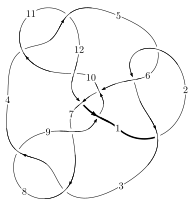
\includegraphics[width=112pt]{../../../GIT/diagram.site/Diagrams/png/1124_12a_0323.png}\\
\ \ \ A knot diagram\footnotemark}&
\allowdisplaybreaks
\textbf{Linearized knot diagam} \\
\cline{2-2}
 &
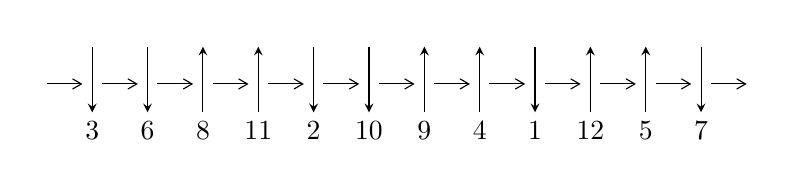
\begin{tikzpicture}[x=20pt, y=17pt]
	% nodes
	\node (C0) at (0, 0) {};
	\node (C1) at (1, 0) {};
	\node (C1U) at (1, +1) {};
	\node (C1D) at (1, -1) {3};

	\node (C2) at (2, 0) {};
	\node (C2U) at (2, +1) {};
	\node (C2D) at (2, -1) {6};

	\node (C3) at (3, 0) {};
	\node (C3U) at (3, +1) {};
	\node (C3D) at (3, -1) {8};

	\node (C4) at (4, 0) {};
	\node (C4U) at (4, +1) {};
	\node (C4D) at (4, -1) {11};

	\node (C5) at (5, 0) {};
	\node (C5U) at (5, +1) {};
	\node (C5D) at (5, -1) {2};

	\node (C6) at (6, 0) {};
	\node (C6U) at (6, +1) {};
	\node (C6D) at (6, -1) {10};

	\node (C7) at (7, 0) {};
	\node (C7U) at (7, +1) {};
	\node (C7D) at (7, -1) {9};

	\node (C8) at (8, 0) {};
	\node (C8U) at (8, +1) {};
	\node (C8D) at (8, -1) {4};

	\node (C9) at (9, 0) {};
	\node (C9U) at (9, +1) {};
	\node (C9D) at (9, -1) {1};

	\node (C10) at (10, 0) {};
	\node (C10U) at (10, +1) {};
	\node (C10D) at (10, -1) {12};

	\node (C11) at (11, 0) {};
	\node (C11U) at (11, +1) {};
	\node (C11D) at (11, -1) {5};

	\node (C12) at (12, 0) {};
	\node (C12U) at (12, +1) {};
	\node (C12D) at (12, -1) {7};
	\node (C13) at (13, 0) {};

	% arrows
	\draw[->,>={angle 60}]
	(C0) edge (C1) (C1) edge (C2) (C2) edge (C3) (C3) edge (C4) (C4) edge (C5) (C5) edge (C6) (C6) edge (C7) (C7) edge (C8) (C8) edge (C9) (C9) edge (C10) (C10) edge (C11) (C11) edge (C12) (C12) edge (C13) ;	\draw[->,>=stealth]
	(C1U) edge (C1D) (C2U) edge (C2D) (C3D) edge (C3U) (C4D) edge (C4U) (C5U) edge (C5D) (C6U) edge (C6D) (C7D) edge (C7U) (C8D) edge (C8U) (C9U) edge (C9D) (C10D) edge (C10U) (C11D) edge (C11U) (C12U) edge (C12D) ;
	\end{tikzpicture} \\
\hhline{~~} \\& 
\textbf{Solving Sequence} \\ \cline{2-2} 
 &
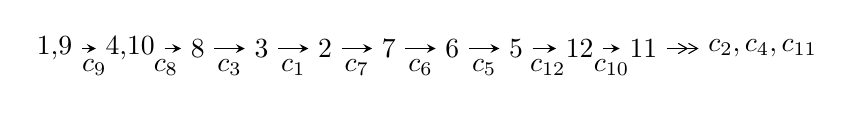
\begin{tikzpicture}[x=23pt, y=7pt]
	% node
	\node (A0) at (-1/8, 0) {1,9};
	\node (A1) at (17/16, 0) {4,10};
	\node (A2) at (17/8, 0) {8};
	\node (A3) at (25/8, 0) {3};
	\node (A4) at (33/8, 0) {2};
	\node (A5) at (41/8, 0) {7};
	\node (A6) at (49/8, 0) {6};
	\node (A7) at (57/8, 0) {5};
	\node (A8) at (65/8, 0) {12};
	\node (A9) at (73/8, 0) {11};
	\node (C1) at (1/2, -1) {$c_{9}$};
	\node (C2) at (13/8, -1) {$c_{8}$};
	\node (C3) at (21/8, -1) {$c_{3}$};
	\node (C4) at (29/8, -1) {$c_{1}$};
	\node (C5) at (37/8, -1) {$c_{7}$};
	\node (C6) at (45/8, -1) {$c_{6}$};
	\node (C7) at (53/8, -1) {$c_{5}$};
	\node (C8) at (61/8, -1) {$c_{12}$};
	\node (C9) at (69/8, -1) {$c_{10}$};
	\node (A10) at (11, 0) {$c_{2},c_{4},c_{11}$};

	% edge
	\draw[->,>=stealth]	
	(A0) edge (A1) (A1) edge (A2) (A2) edge (A3) (A3) edge (A4) (A4) edge (A5) (A5) edge (A6) (A6) edge (A7) (A7) edge (A8) (A8) edge (A9) ;
	\draw[->>,>={angle 60}]	
	(A9) edge (A10);
\end{tikzpicture} \\ 

\end{tabular} \\

\footnotetext{
The image of knot diagram is generated by the software ``\textbf{Draw programme}" developed by Andrew Bartholomew(\url{http://www.layer8.co.uk/maths/draw/index.htm\#Running-draw}), where we modified some parts for our purpose(\url{https://github.com/CATsTAILs/LinksPainter}).
}\phantom \\ \newline 
\centering \textbf{Ideals for irreducible components\footnotemark of $X_{\text{par}}$} 
 
\begin{align*}
I^u_{1}&=\langle 
6.55331\times10^{30} u^{30}+1.64150\times10^{31} u^{29}+\cdots+3.56183\times10^{31} b+4.47272\times10^{31},\\
\phantom{I^u_{1}}&\phantom{= \langle  }1.84263\times10^{31} u^{30}+6.93262\times10^{29} u^{29}+\cdots+3.56183\times10^{31} a+6.39301\times10^{31},\;u^{31}+u^{30}+\cdots+4 u^2+1\rangle \\
I^u_{2}&=\langle 
-5.81751\times10^{941} u^{125}+8.58847\times10^{942} u^{124}+\cdots+3.92230\times10^{942} b-1.21679\times10^{942},\\
\phantom{I^u_{2}}&\phantom{= \langle  }-2.73119\times10^{942} u^{125}+4.02364\times10^{943} u^{124}+\cdots+3.92230\times10^{942} a-5.31484\times10^{943},\\
\phantom{I^u_{2}}&\phantom{= \langle  }u^{126}-15 u^{125}+\cdots-10 u+1\rangle \\
I^u_{3}&=\langle 
u^9- u^7- u^6- u^5+u^3+b+u,\;u^{14}+2 u^{13}-2 u^{11}-4 u^{10}-4 u^9+2 u^7+2 u^6+3 u^5- u^2+a,\\
\phantom{I^u_{3}}&\phantom{= \langle  }u^{15}+u^{14}- u^{12}-3 u^{11}-3 u^{10}- u^9+3 u^7+3 u^6+2 u^5+u^4- u^3- u^2- u-1\rangle \\
I^u_{4}&=\langle 
u^{15}+2 u^{14}-2 u^{13}-5 u^{12}+2 u^{11}+6 u^{10}-3 u^9-8 u^8+u^7+3 u^6+u^4-2 u^2+b-2 u+3,\\
\phantom{I^u_{4}}&\phantom{= \langle  }-14 u^{15}-10 u^{14}+\cdots+a+18,\\
\phantom{I^u_{4}}&\phantom{= \langle  }u^{16}-3 u^{14}+2 u^{13}+4 u^{12}-3 u^{11}-4 u^{10}+4 u^9+3 u^8-6 u^7+5 u^6-3 u^5+2 u^4-4 u^3+6 u^2-4 u+1\rangle \\
\\
\end{align*}
\raggedright * 4 irreducible components of $\dim_{\mathbb{C}}=0$, with total 188 representations.\\
\footnotetext{All coefficients of polynomials are rational numbers. But the coefficients are sometimes approximated in decimal forms when there is not enough margin.}
\newpage
\renewcommand{\arraystretch}{1}
\centering \section*{I. $I^u_{1}= \langle 6.55\times10^{30} u^{30}+1.64\times10^{31} u^{29}+\cdots+3.56\times10^{31} b+4.47\times10^{31},\;1.84\times10^{31} u^{30}+6.93\times10^{29} u^{29}+\cdots+3.56\times10^{31} a+6.39\times10^{31},\;u^{31}+u^{30}+\cdots+4 u^2+1 \rangle$}
\flushleft \textbf{(i) Arc colorings}\\
\begin{tabular}{m{7pt} m{180pt} m{7pt} m{180pt} }
\flushright $a_{1}=$&$\begin{pmatrix}0\\u\end{pmatrix}$ \\
\flushright $a_{9}=$&$\begin{pmatrix}1\\0\end{pmatrix}$ \\
\flushright $a_{4}=$&$\begin{pmatrix}-0.517327 u^{30}-0.0194636 u^{29}+\cdots-5.01519 u-1.79487\\-0.183987 u^{30}-0.460859 u^{29}+\cdots-0.222841 u-1.25573\end{pmatrix}$ \\
\flushright $a_{10}=$&$\begin{pmatrix}1\\u^2\end{pmatrix}$ \\
\flushright $a_{8}=$&$\begin{pmatrix}0.216938 u^{30}+0.559109 u^{29}+\cdots+4.24716 u+0.409583\\-0.127744 u^{30}+0.156322 u^{29}+\cdots+0.655318 u-0.0581050\end{pmatrix}$ \\
\flushright $a_{3}=$&$\begin{pmatrix}0.608908 u^{30}+0.513421 u^{29}+\cdots-0.141955 u-2.34677\\0.437378 u^{30}+0.0595317 u^{29}+\cdots+0.528023 u-0.947344\end{pmatrix}$ \\
\flushright $a_{2}=$&$\begin{pmatrix}1.55810 u^{30}+0.725606 u^{29}+\cdots-3.80603 u-2.48799\\0.329814 u^{30}-0.151160 u^{29}+\cdots-1.45162 u-0.00731807\end{pmatrix}$ \\
\flushright $a_{7}=$&$\begin{pmatrix}0.344682 u^{30}+0.402787 u^{29}+\cdots+3.59184 u+0.467688\\-0.127744 u^{30}+0.156322 u^{29}+\cdots+0.655318 u-0.0581050\end{pmatrix}$ \\
\flushright $a_{6}=$&$\begin{pmatrix}0.344682 u^{30}+0.402787 u^{29}+\cdots+4.59184 u+0.467688\\-0.127744 u^{30}+0.156322 u^{29}+\cdots+0.655318 u-0.0581050\end{pmatrix}$ \\
\flushright $a_{5}=$&$\begin{pmatrix}2.15136 u^{30}+0.404329 u^{29}+\cdots-1.94509 u-1.88658\\0.440312 u^{30}+0.351852 u^{29}+\cdots-1.62334 u+0.799685\end{pmatrix}$ \\
\flushright $a_{12}=$&$\begin{pmatrix}1.06778 u^{30}+1.15510 u^{29}+\cdots+6.10440 u-1.82049\\0.0239911 u^{30}-0.155795 u^{29}+\cdots-0.412459 u-0.145425\end{pmatrix}$ \\
\flushright $a_{11}=$&$\begin{pmatrix}0.182230 u^{30}+0.115877 u^{29}+\cdots-3.91942 u+3.96267\\0.266137 u^{30}+0.197519 u^{29}+\cdots+0.0212995 u-0.0373999\end{pmatrix}$\\&\end{tabular}
\flushleft \textbf{(ii) Obstruction class $= -1$}\\~\\
\flushleft \textbf{(iii) Cusp Shapes $= 0.100681 u^{30}+1.00392 u^{29}+\cdots-7.27867 u+2.00104$}\\~\\
\newpage\renewcommand{\arraystretch}{1}
\flushleft \textbf{(iv) u-Polynomials at the component}\newline \\
\begin{tabular}{m{50pt}|m{274pt}}
Crossings & \hspace{64pt}u-Polynomials at each crossing \\
\hline $$\begin{aligned}c_{1}\end{aligned}$$&$\begin{aligned}
&u^{31}+12 u^{30}+\cdots+5632 u+1024
\end{aligned}$\\
\hline $$\begin{aligned}c_{2},c_{5}\end{aligned}$$&$\begin{aligned}
&u^{31}+12 u^{30}+\cdots-224 u-32
\end{aligned}$\\
\hline $$\begin{aligned}c_{3},c_{4},c_{8}\\c_{11}\end{aligned}$$&$\begin{aligned}
&u^{31}-7 u^{29}+\cdots+3 u+1
\end{aligned}$\\
\hline $$\begin{aligned}c_{6},c_{9}\end{aligned}$$&$\begin{aligned}
&u^{31}+u^{30}+\cdots+4 u^2+1
\end{aligned}$\\
\hline $$\begin{aligned}c_{7},c_{10}\end{aligned}$$&$\begin{aligned}
&u^{31}-14 u^{30}+\cdots+11 u-1
\end{aligned}$\\
\hline $$\begin{aligned}c_{12}\end{aligned}$$&$\begin{aligned}
&u^{31}+28 u^{30}+\cdots+116736 u+10240
\end{aligned}$\\
\hline
\end{tabular}\\~\\
\newpage\renewcommand{\arraystretch}{1}
\flushleft \textbf{(v) Riley Polynomials at the component}\newline \\
\begin{tabular}{m{50pt}|m{274pt}}
Crossings & \hspace{64pt}Riley Polynomials at each crossing \\
\hline $$\begin{aligned}c_{1}\end{aligned}$$&$\begin{aligned}
&y^{31}+12 y^{30}+\cdots-393216 y-1048576
\end{aligned}$\\
\hline $$\begin{aligned}c_{2},c_{5}\end{aligned}$$&$\begin{aligned}
&y^{31}-12 y^{30}+\cdots+5632 y-1024
\end{aligned}$\\
\hline $$\begin{aligned}c_{3},c_{4},c_{8}\\c_{11}\end{aligned}$$&$\begin{aligned}
&y^{31}-14 y^{30}+\cdots+11 y-1
\end{aligned}$\\
\hline $$\begin{aligned}c_{6},c_{9}\end{aligned}$$&$\begin{aligned}
&y^{31}+5 y^{30}+\cdots-8 y-1
\end{aligned}$\\
\hline $$\begin{aligned}c_{7},c_{10}\end{aligned}$$&$\begin{aligned}
&y^{31}+10 y^{30}+\cdots+95 y-1
\end{aligned}$\\
\hline $$\begin{aligned}c_{12}\end{aligned}$$&$\begin{aligned}
&y^{31}-8 y^{30}+\cdots+69206016 y-104857600
\end{aligned}$\\
\hline
\end{tabular}\\~\\
\newpage\flushleft \textbf{(vi) Complex Volumes and Cusp Shapes}
$$\begin{array}{c|c|c}  
\text{Solutions to }I^u_{1}& \I (\text{vol} + \sqrt{-1}CS) & \text{Cusp shape}\\
 \hline 
\begin{aligned}
u &= \phantom{-}0.084144 + 1.039664 I \\
a &= -1.269352 + 0.109533 I \\
b &= \phantom{-}0.962289 - 0.520246 I\end{aligned}
 & \phantom{-}3.19876 - 7.55195 I & \phantom{-}5.48862 + 9.87953 I \\ \hline\begin{aligned}
u &= \phantom{-}0.084144 - 1.039664 I \\
a &= -1.269352 - 0.109533 I \\
b &= \phantom{-}0.962289 + 0.520246 I\end{aligned}
 & \phantom{-}3.19876 + 7.55195 I & \phantom{-}5.48862 - 9.87953 I \\ \hline\begin{aligned}
u &= -0.469459 + 1.009713 I \\
a &= \phantom{-}0.218341 - 0.735028 I \\
b &= -0.879624 + 0.475488 I\end{aligned}
 & \phantom{-}2.43175 - 0.36874 I & \phantom{-}2.25000 + 2.94789 I \\ \hline\begin{aligned}
u &= -0.469459 - 1.009713 I \\
a &= \phantom{-}0.218341 + 0.735028 I \\
b &= -0.879624 - 0.475488 I\end{aligned}
 & \phantom{-}2.43175 + 0.36874 I & \phantom{-}2.25000 - 2.94789 I \\ \hline\begin{aligned}
u &= \phantom{-}0.860162 + 0.786995 I \\
a &= \phantom{-}0.78085 + 1.82232 I \\
b &= -1.020462 + 0.682561 I\end{aligned}
 & -5.34193 - 10.63260 I & -3.15069 + 9.70062 I \\ \hline\begin{aligned}
u &= \phantom{-}0.860162 - 0.786995 I \\
a &= \phantom{-}0.78085 - 1.82232 I \\
b &= -1.020462 - 0.682561 I\end{aligned}
 & -5.34193 + 10.63260 I & -3.15069 - 9.70062 I \\ \hline\begin{aligned}
u &= -1.21341\phantom{ +0.000000I} \\
a &= -0.0217834\phantom{ +0.000000I} \\
b &= -0.330185\phantom{ +0.000000I}\end{aligned}
 & -2.42715\phantom{ +0.000000I} & -5.31520\phantom{ +0.000000I} \\ \hline\begin{aligned}
u &= \phantom{-}0.387802 + 1.194509 I \\
a &= \phantom{-}0.298582 - 0.479894 I \\
b &= -1.157971 - 0.198479 I\end{aligned}
 & \phantom{-}8.01085 + 1.87526 I & \phantom{-}9.36813 - 2.63874 I \\ \hline\begin{aligned}
u &= \phantom{-}0.387802 - 1.194509 I \\
a &= \phantom{-}0.298582 + 0.479894 I \\
b &= -1.157971 + 0.198479 I\end{aligned}
 & \phantom{-}8.01085 - 1.87526 I & \phantom{-}9.36813 + 2.63874 I \\ \hline\begin{aligned}
u &= -1.117652 + 0.663220 I \\
a &= \phantom{-}0.785976 - 0.601863 I \\
b &= \phantom{-}0.695306 - 0.761608 I\end{aligned}
 & -7.37204 - 0.41255 I & -6.92882 + 2.19694 I\\
 \hline 
 \end{array}$$\newpage$$\begin{array}{c|c|c}  
\text{Solutions to }I^u_{1}& \I (\text{vol} + \sqrt{-1}CS) & \text{Cusp shape}\\
 \hline 
\begin{aligned}
u &= -1.117652 - 0.663220 I \\
a &= \phantom{-}0.785976 + 0.601863 I \\
b &= \phantom{-}0.695306 + 0.761608 I\end{aligned}
 & -7.37204 + 0.41255 I & -6.92882 - 2.19694 I \\ \hline\begin{aligned}
u &= -0.534239 + 0.421201 I \\
a &= \phantom{-}0.94640 + 3.61057 I \\
b &= \phantom{-}1.042485 + 0.517986 I\end{aligned}
 & \phantom{-}0.94025 + 10.62460 I & \phantom{-}2.5262 - 14.8925 I \\ \hline\begin{aligned}
u &= -0.534239 - 0.421201 I \\
a &= \phantom{-}0.94640 - 3.61057 I \\
b &= \phantom{-}1.042485 - 0.517986 I\end{aligned}
 & \phantom{-}0.94025 - 10.62460 I & \phantom{-}2.5262 + 14.8925 I \\ \hline\begin{aligned}
u &= -1.007284 + 0.875628 I \\
a &= -0.307838 + 0.750851 I \\
b &= -0.484729 + 0.824665 I\end{aligned}
 & -2.35818 + 2.80518 I & -2.26135 - 0.49699 I \\ \hline\begin{aligned}
u &= -1.007284 - 0.875628 I \\
a &= -0.307838 - 0.750851 I \\
b &= -0.484729 - 0.824665 I\end{aligned}
 & -2.35818 - 2.80518 I & -2.26135 + 0.49699 I \\ \hline\begin{aligned}
u &= -0.416545 + 0.469850 I \\
a &= \phantom{-}0.614182 + 0.161827 I \\
b &= -0.022556 + 0.572988 I\end{aligned}
 & -0.57873 + 1.51038 I & -2.67375 - 4.66317 I \\ \hline\begin{aligned}
u &= -0.416545 - 0.469850 I \\
a &= \phantom{-}0.614182 - 0.161827 I \\
b &= -0.022556 - 0.572988 I\end{aligned}
 & -0.57873 - 1.51038 I & -2.67375 + 4.66317 I \\ \hline\begin{aligned}
u &= \phantom{-}0.652733 + 1.249388 I \\
a &= -0.189535 + 0.299518 I \\
b &= \phantom{-}1.153307 + 0.140718 I\end{aligned}
 & \phantom{-}7.25146 - 3.68008 I & \phantom{-}8.25009 + 3.16950 I \\ \hline\begin{aligned}
u &= \phantom{-}0.652733 - 1.249388 I \\
a &= -0.189535 - 0.299518 I \\
b &= \phantom{-}1.153307 - 0.140718 I\end{aligned}
 & \phantom{-}7.25146 + 3.68008 I & \phantom{-}8.25009 - 3.16950 I \\ \hline\begin{aligned}
u &= -0.135838 + 0.563252 I \\
a &= \phantom{-}2.18955 - 2.36363 I \\
b &= -1.026841 - 0.393178 I\end{aligned}
 & \phantom{-}4.55871 + 4.50370 I & \phantom{-}11.51940 - 4.92639 I\\
 \hline 
 \end{array}$$\newpage$$\begin{array}{c|c|c}  
\text{Solutions to }I^u_{1}& \I (\text{vol} + \sqrt{-1}CS) & \text{Cusp shape}\\
 \hline 
\begin{aligned}
u &= -0.135838 - 0.563252 I \\
a &= \phantom{-}2.18955 + 2.36363 I \\
b &= -1.026841 + 0.393178 I\end{aligned}
 & \phantom{-}4.55871 - 4.50370 I & \phantom{-}11.51940 + 4.92639 I \\ \hline\begin{aligned}
u &= \phantom{-}0.419041 + 0.284363 I \\
a &= \phantom{-}0.070359 - 1.058717 I \\
b &= \phantom{-}0.882191 + 0.161261 I\end{aligned}
 & \phantom{-}1.83304 + 0.30388 I & \phantom{-}4.09035 + 0.14569 I \\ \hline\begin{aligned}
u &= \phantom{-}0.419041 - 0.284363 I \\
a &= \phantom{-}0.070359 + 1.058717 I \\
b &= \phantom{-}0.882191 - 0.161261 I\end{aligned}
 & \phantom{-}1.83304 - 0.30388 I & \phantom{-}4.09035 - 0.14569 I \\ \hline\begin{aligned}
u &= -1.13002 + 0.99523 I \\
a &= \phantom{-}0.384328 - 0.974043 I \\
b &= \phantom{-}0.524500 - 0.942497 I\end{aligned}
 & -4.76248 + 7.98624 I & -4.49283 - 4.44036 I \\ \hline\begin{aligned}
u &= -1.13002 - 0.99523 I \\
a &= \phantom{-}0.384328 + 0.974043 I \\
b &= \phantom{-}0.524500 + 0.942497 I\end{aligned}
 & -4.76248 - 7.98624 I & -4.49283 + 4.44036 I \\ \hline\begin{aligned}
u &= \phantom{-}0.258738 + 0.349549 I \\
a &= -2.82094 - 1.20057 I \\
b &= -0.470895 - 0.606546 I\end{aligned}
 & -2.41931 - 1.71382 I & -3.05380 + 2.44778 I \\ \hline\begin{aligned}
u &= \phantom{-}0.258738 - 0.349549 I \\
a &= -2.82094 + 1.20057 I \\
b &= -0.470895 + 0.606546 I\end{aligned}
 & -2.41931 + 1.71382 I & -3.05380 - 2.44778 I \\ \hline\begin{aligned}
u &= \phantom{-}1.03795 + 1.17821 I \\
a &= -0.317255 - 1.306538 I \\
b &= \phantom{-}1.129177 - 0.655726 I\end{aligned}
 & \phantom{-}1.52020 - 14.00050 I & \phantom{-}2.53500 + 8.42876 I \\ \hline\begin{aligned}
u &= \phantom{-}1.03795 - 1.17821 I \\
a &= -0.317255 + 1.306538 I \\
b &= \phantom{-}1.129177 + 0.655726 I\end{aligned}
 & \phantom{-}1.52020 + 14.00050 I & \phantom{-}2.53500 - 8.42876 I \\ \hline\begin{aligned}
u &= \phantom{-}1.21717 + 1.17818 I \\
a &= \phantom{-}0.127234 + 1.383611 I \\
b &= -1.161086 + 0.692549 I\end{aligned}
 & -0.7640 - 20.0875 I & \phantom{-0.000000 -}0. + 11.57868 I\\
 \hline 
 \end{array}$$\newpage$$\begin{array}{c|c|c}  
\text{Solutions to }I^u_{1}& \I (\text{vol} + \sqrt{-1}CS) & \text{Cusp shape}\\
 \hline 
\begin{aligned}
u &= \phantom{-}1.21717 - 1.17818 I \\
a &= \phantom{-}0.127234 - 1.383611 I \\
b &= -1.161086 - 0.692549 I\end{aligned}
 & -0.7640 + 20.0875 I & \phantom{-0.000000 } 0. - 11.57868 I\\
 \hline 
 \end{array}$$\newpage\newpage\renewcommand{\arraystretch}{1}
\centering \section*{II. $I^u_{2}= \langle -5.82\times10^{941} u^{125}+8.59\times10^{942} u^{124}+\cdots+3.92\times10^{942} b-1.22\times10^{942},\;-2.73\times10^{942} u^{125}+4.02\times10^{943} u^{124}+\cdots+3.92\times10^{942} a-5.31\times10^{943},\;u^{126}-15 u^{125}+\cdots-10 u+1 \rangle$}
\flushleft \textbf{(i) Arc colorings}\\
\begin{tabular}{m{7pt} m{180pt} m{7pt} m{180pt} }
\flushright $a_{1}=$&$\begin{pmatrix}0\\u\end{pmatrix}$ \\
\flushright $a_{9}=$&$\begin{pmatrix}1\\0\end{pmatrix}$ \\
\flushright $a_{4}=$&$\begin{pmatrix}0.696323 u^{125}-10.2584 u^{124}+\cdots-66.3738 u+13.5503\\0.148319 u^{125}-2.18965 u^{124}+\cdots-0.702479 u+0.310223\end{pmatrix}$ \\
\flushright $a_{10}=$&$\begin{pmatrix}1\\u^2\end{pmatrix}$ \\
\flushright $a_{8}=$&$\begin{pmatrix}-0.0582623 u^{125}+0.933870 u^{124}+\cdots-143.836 u+13.2497\\-0.161908 u^{125}+2.39661 u^{124}+\cdots-12.9534 u+0.956689\end{pmatrix}$ \\
\flushright $a_{3}=$&$\begin{pmatrix}1.54346 u^{125}-23.0357 u^{124}+\cdots+124.214 u+1.81945\\0.204893 u^{125}-3.05880 u^{124}+\cdots+12.9608 u-0.797883\end{pmatrix}$ \\
\flushright $a_{2}=$&$\begin{pmatrix}0.615790 u^{125}-9.03866 u^{124}+\cdots-104.459 u+15.5686\\0.228570 u^{125}-3.39770 u^{124}+\cdots+1.58590 u-0.205166\end{pmatrix}$ \\
\flushright $a_{7}=$&$\begin{pmatrix}0.103646 u^{125}-1.46274 u^{124}+\cdots-130.883 u+12.2930\\-0.161908 u^{125}+2.39661 u^{124}+\cdots-12.9534 u+0.956689\end{pmatrix}$ \\
\flushright $a_{6}=$&$\begin{pmatrix}-0.0448889 u^{125}+0.738359 u^{124}+\cdots-144.652 u+13.3417\\-0.173193 u^{125}+2.55966 u^{124}+\cdots-13.0741 u+0.983617\end{pmatrix}$ \\
\flushright $a_{5}=$&$\begin{pmatrix}0.645712 u^{125}-9.65714 u^{124}+\cdots+84.5594 u-3.82633\\0.0274567 u^{125}-0.441852 u^{124}+\cdots+5.88458 u-0.629101\end{pmatrix}$ \\
\flushright $a_{12}=$&$\begin{pmatrix}0.758231 u^{125}-11.2624 u^{124}+\cdots-32.2325 u+13.3940\\0.105098 u^{125}-1.56250 u^{124}+\cdots-0.481745 u+0.633800\end{pmatrix}$ \\
\flushright $a_{11}=$&$\begin{pmatrix}-0.617167 u^{125}+9.10795 u^{124}+\cdots+100.828 u-14.9786\\-0.0878400 u^{125}+1.30605 u^{124}+\cdots+5.74816 u-0.594280\end{pmatrix}$\\&\end{tabular}
\flushleft \textbf{(ii) Obstruction class $= -1$}\\~\\
\flushleft \textbf{(iii) Cusp Shapes $= 1.18500 u^{125}-17.5443 u^{124}+\cdots+35.1425 u-2.66616$}\\~\\
\newpage\renewcommand{\arraystretch}{1}
\flushleft \textbf{(iv) u-Polynomials at the component}\newline \\
\begin{tabular}{m{50pt}|m{274pt}}
Crossings & \hspace{64pt}u-Polynomials at each crossing \\
\hline $$\begin{aligned}c_{1}\end{aligned}$$&$\begin{aligned}
&(u^{63}+29 u^{62}+\cdots+399 u+25)^{2}
\end{aligned}$\\
\hline $$\begin{aligned}c_{2},c_{5}\end{aligned}$$&$\begin{aligned}
&(u^{63}-5 u^{62}+\cdots+37 u-5)^{2}
\end{aligned}$\\
\hline $$\begin{aligned}c_{3},c_{4},c_{8}\\c_{11}\end{aligned}$$&$\begin{aligned}
&u^{126}+u^{125}+\cdots+36 u+9
\end{aligned}$\\
\hline $$\begin{aligned}c_{6},c_{9}\end{aligned}$$&$\begin{aligned}
&u^{126}-15 u^{125}+\cdots-10 u+1
\end{aligned}$\\
\hline $$\begin{aligned}c_{7},c_{10}\end{aligned}$$&$\begin{aligned}
&u^{126}-53 u^{125}+\cdots-2628 u+81
\end{aligned}$\\
\hline $$\begin{aligned}c_{12}\end{aligned}$$&$\begin{aligned}
&(u^{63}-13 u^{62}+\cdots-5 u+1)^{2}
\end{aligned}$\\
\hline
\end{tabular}\\~\\
\newpage\renewcommand{\arraystretch}{1}
\flushleft \textbf{(v) Riley Polynomials at the component}\newline \\
\begin{tabular}{m{50pt}|m{274pt}}
Crossings & \hspace{64pt}Riley Polynomials at each crossing \\
\hline $$\begin{aligned}c_{1}\end{aligned}$$&$\begin{aligned}
&(y^{63}+19 y^{62}+\cdots+4651 y-625)^{2}
\end{aligned}$\\
\hline $$\begin{aligned}c_{2},c_{5}\end{aligned}$$&$\begin{aligned}
&(y^{63}-29 y^{62}+\cdots+399 y-25)^{2}
\end{aligned}$\\
\hline $$\begin{aligned}c_{3},c_{4},c_{8}\\c_{11}\end{aligned}$$&$\begin{aligned}
&y^{126}-53 y^{125}+\cdots-2628 y+81
\end{aligned}$\\
\hline $$\begin{aligned}c_{6},c_{9}\end{aligned}$$&$\begin{aligned}
&y^{126}-15 y^{125}+\cdots+248 y+1
\end{aligned}$\\
\hline $$\begin{aligned}c_{7},c_{10}\end{aligned}$$&$\begin{aligned}
&y^{126}+51 y^{125}+\cdots+935388 y+6561
\end{aligned}$\\
\hline $$\begin{aligned}c_{12}\end{aligned}$$&$\begin{aligned}
&(y^{63}-15 y^{62}+\cdots+49 y-1)^{2}
\end{aligned}$\\
\hline
\end{tabular}\\~\\
\newpage\flushleft \textbf{(vi) Complex Volumes and Cusp Shapes}
$$\begin{array}{c|c|c}  
\text{Solutions to }I^u_{2}& \I (\text{vol} + \sqrt{-1}CS) & \text{Cusp shape}\\
 \hline 
\begin{aligned}
u &= -1.041871 + 0.086991 I \\
a &= \phantom{-}0.106651 + 0.659044 I \\
b &= -0.196963 + 0.634548 I\end{aligned}
 & -2.40615 + 0.01706 I & \phantom{-0.000000 } 0 \\ \hline\begin{aligned}
u &= -1.041871 - 0.086991 I \\
a &= \phantom{-}0.106651 - 0.659044 I \\
b &= -0.196963 - 0.634548 I\end{aligned}
 & -2.40615 - 0.01706 I & \phantom{-0.000000 } 0 \\ \hline\begin{aligned}
u &= \phantom{-}0.447529 + 0.839925 I \\
a &= \phantom{-}0.529540 - 0.312626 I \\
b &= -1.275041 - 0.062031 I\end{aligned}
 & \phantom{-}5.57710 - 5.64020 I & \phantom{-0.000000 } 0 \\ \hline\begin{aligned}
u &= \phantom{-}0.447529 - 0.839925 I \\
a &= \phantom{-}0.529540 + 0.312626 I \\
b &= -1.275041 + 0.062031 I\end{aligned}
 & \phantom{-}5.57710 + 5.64020 I & \phantom{-0.000000 } 0 \\ \hline\begin{aligned}
u &= -0.904169 + 0.533833 I \\
a &= \phantom{-}0.002039 - 1.079744 I \\
b &= -1.196784 - 0.631391 I\end{aligned}
 & \phantom{-}0.38539 + 5.30492 I & \phantom{-0.000000 } 0 \\ \hline\begin{aligned}
u &= -0.904169 - 0.533833 I \\
a &= \phantom{-}0.002039 + 1.079744 I \\
b &= -1.196784 + 0.631391 I\end{aligned}
 & \phantom{-}0.38539 - 5.30492 I & \phantom{-0.000000 } 0 \\ \hline\begin{aligned}
u &= -0.931507 + 0.182036 I \\
a &= \phantom{-}0.140837 + 1.105782 I \\
b &= \phantom{-}0.220517 + 1.076032 I\end{aligned}
 & -3.86874 - 3.84740 I & \phantom{-0.000000 } 0 \\ \hline\begin{aligned}
u &= -0.931507 - 0.182036 I \\
a &= \phantom{-}0.140837 - 1.105782 I \\
b &= \phantom{-}0.220517 - 1.076032 I\end{aligned}
 & -3.86874 + 3.84740 I & \phantom{-0.000000 } 0 \\ \hline\begin{aligned}
u &= -0.883551 + 0.346025 I \\
a &= -0.16505 + 1.54628 I \\
b &= \phantom{-}1.193652 + 0.560788 I\end{aligned}
 & \phantom{-}0.81103 + 4.65824 I & \phantom{-0.000000 } 0 \\ \hline\begin{aligned}
u &= -0.883551 - 0.346025 I \\
a &= -0.16505 - 1.54628 I \\
b &= \phantom{-}1.193652 - 0.560788 I\end{aligned}
 & \phantom{-}0.81103 - 4.65824 I & \phantom{-0.000000 } 0\\
 \hline 
 \end{array}$$\newpage$$\begin{array}{c|c|c}  
\text{Solutions to }I^u_{2}& \I (\text{vol} + \sqrt{-1}CS) & \text{Cusp shape}\\
 \hline 
\begin{aligned}
u &= \phantom{-}0.828283 + 0.446669 I \\
a &= \phantom{-}0.069163 - 1.144444 I \\
b &= \phantom{-}1.072744 - 0.653846 I\end{aligned}
 & \phantom{-}0.067312 - 1.017350 I & \phantom{-0.000000 } 0 \\ \hline\begin{aligned}
u &= \phantom{-}0.828283 - 0.446669 I \\
a &= \phantom{-}0.069163 + 1.144444 I \\
b &= \phantom{-}1.072744 + 0.653846 I\end{aligned}
 & \phantom{-}0.067312 + 1.017350 I & \phantom{-0.000000 } 0 \\ \hline\begin{aligned}
u &= -0.281852 + 1.028357 I \\
a &= \phantom{-}0.641319 - 0.218069 I \\
b &= -1.088591 - 0.334536 I\end{aligned}
 & \phantom{-}2.50341 + 4.73463 I & \phantom{-0.000000 } 0 \\ \hline\begin{aligned}
u &= -0.281852 - 1.028357 I \\
a &= \phantom{-}0.641319 + 0.218069 I \\
b &= -1.088591 + 0.334536 I\end{aligned}
 & \phantom{-}2.50341 - 4.73463 I & \phantom{-0.000000 } 0 \\ \hline\begin{aligned}
u &= \phantom{-}0.461999 + 0.809904 I \\
a &= -0.283438 - 0.866112 I \\
b &= \phantom{-}1.029079 + 0.162258 I\end{aligned}
 & \phantom{-}1.82989 + 0.00826 I & \phantom{-0.000000 } 0 \\ \hline\begin{aligned}
u &= \phantom{-}0.461999 - 0.809904 I \\
a &= -0.283438 + 0.866112 I \\
b &= \phantom{-}1.029079 - 0.162258 I\end{aligned}
 & \phantom{-}1.82989 - 0.00826 I & \phantom{-0.000000 } 0 \\ \hline\begin{aligned}
u &= -0.525617 + 0.937016 I \\
a &= \phantom{-}0.226511 - 0.805413 I \\
b &= -1.045075 + 0.320939 I\end{aligned}
 & \phantom{-}2.19990 + 4.01790 I & \phantom{-0.000000 } 0 \\ \hline\begin{aligned}
u &= -0.525617 - 0.937016 I \\
a &= \phantom{-}0.226511 + 0.805413 I \\
b &= -1.045075 - 0.320939 I\end{aligned}
 & \phantom{-}2.19990 - 4.01790 I & \phantom{-0.000000 } 0 \\ \hline\begin{aligned}
u &= \phantom{-}0.916902 + 0.019751 I \\
a &= \phantom{-}0.154113 + 0.799212 I \\
b &= \phantom{-}0.565274 + 0.789159 I\end{aligned}
 & -1.50295 + 4.40389 I & \phantom{-0.000000 } 0 \\ \hline\begin{aligned}
u &= \phantom{-}0.916902 - 0.019751 I \\
a &= \phantom{-}0.154113 - 0.799212 I \\
b &= \phantom{-}0.565274 - 0.789159 I\end{aligned}
 & -1.50295 - 4.40389 I & \phantom{-0.000000 } 0\\
 \hline 
 \end{array}$$\newpage$$\begin{array}{c|c|c}  
\text{Solutions to }I^u_{2}& \I (\text{vol} + \sqrt{-1}CS) & \text{Cusp shape}\\
 \hline 
\begin{aligned}
u &= \phantom{-}0.430967 + 0.997335 I \\
a &= -0.240799 - 0.693857 I \\
b &= \phantom{-}0.725649 + 0.459266 I\end{aligned}
 & \phantom{-}2.37286 - 3.46728 I & \phantom{-0.000000 } 0 \\ \hline\begin{aligned}
u &= \phantom{-}0.430967 - 0.997335 I \\
a &= -0.240799 + 0.693857 I \\
b &= \phantom{-}0.725649 - 0.459266 I\end{aligned}
 & \phantom{-}2.37286 + 3.46728 I & \phantom{-0.000000 } 0 \\ \hline\begin{aligned}
u &= -0.115187 + 1.081445 I \\
a &= \phantom{-}1.100285 + 0.181739 I \\
b &= -0.867542 - 0.461944 I\end{aligned}
 & \phantom{-}2.37286 + 3.46728 I & \phantom{-0.000000 } 0 \\ \hline\begin{aligned}
u &= -0.115187 - 1.081445 I \\
a &= \phantom{-}1.100285 - 0.181739 I \\
b &= -0.867542 + 0.461944 I\end{aligned}
 & \phantom{-}2.37286 - 3.46728 I & \phantom{-0.000000 } 0 \\ \hline\begin{aligned}
u &= -0.265622 + 0.871434 I \\
a &= -0.545305 - 0.493257 I \\
b &= \phantom{-}1.185667 - 0.038115 I\end{aligned}
 & \phantom{-}3.45279 + 0.77574 I & \phantom{-0.000000 } 0 \\ \hline\begin{aligned}
u &= -0.265622 - 0.871434 I \\
a &= -0.545305 + 0.493257 I \\
b &= \phantom{-}1.185667 + 0.038115 I\end{aligned}
 & \phantom{-}3.45279 - 0.77574 I & \phantom{-0.000000 } 0 \\ \hline\begin{aligned}
u &= -0.861309 + 0.257273 I \\
a &= \phantom{-}0.136789 + 1.296927 I \\
b &= \phantom{-}1.26829 + 0.71351 I\end{aligned}
 & -0.74509 + 10.25710 I & \phantom{-0.000000 } 0 \\ \hline\begin{aligned}
u &= -0.861309 - 0.257273 I \\
a &= \phantom{-}0.136789 - 1.296927 I \\
b &= \phantom{-}1.26829 - 0.71351 I\end{aligned}
 & -0.74509 - 10.25710 I & \phantom{-0.000000 } 0 \\ \hline\begin{aligned}
u &= \phantom{-}0.115055 + 0.889723 I \\
a &= -1.50506 - 0.40824 I \\
b &= \phantom{-}1.057783 - 0.452075 I\end{aligned}
 & \phantom{-}4.14790 - 2.17573 I & \phantom{-0.000000 } 0 \\ \hline\begin{aligned}
u &= \phantom{-}0.115055 - 0.889723 I \\
a &= -1.50506 + 0.40824 I \\
b &= \phantom{-}1.057783 + 0.452075 I\end{aligned}
 & \phantom{-}4.14790 + 2.17573 I & \phantom{-0.000000 } 0\\
 \hline 
 \end{array}$$\newpage$$\begin{array}{c|c|c}  
\text{Solutions to }I^u_{2}& \I (\text{vol} + \sqrt{-1}CS) & \text{Cusp shape}\\
 \hline 
\begin{aligned}
u &= \phantom{-}0.890223 + 0.685331 I \\
a &= -0.124561 - 1.005106 I \\
b &= \phantom{-}1.253089 - 0.331609 I\end{aligned}
 & \phantom{-}1.08734 - 5.02241 I & \phantom{-0.000000 } 0 \\ \hline\begin{aligned}
u &= \phantom{-}0.890223 - 0.685331 I \\
a &= -0.124561 + 1.005106 I \\
b &= \phantom{-}1.253089 + 0.331609 I\end{aligned}
 & \phantom{-}1.08734 + 5.02241 I & \phantom{-0.000000 } 0 \\ \hline\begin{aligned}
u &= -0.916222 + 0.653646 I \\
a &= \phantom{-}0.081515 - 1.025750 I \\
b &= -1.289559 - 0.453742 I\end{aligned}
 & \phantom{-}0.89643 + 1.17973 I & \phantom{-0.000000 } 0 \\ \hline\begin{aligned}
u &= -0.916222 - 0.653646 I \\
a &= \phantom{-}0.081515 + 1.025750 I \\
b &= -1.289559 + 0.453742 I\end{aligned}
 & \phantom{-}0.89643 - 1.17973 I & \phantom{-0.000000 } 0 \\ \hline\begin{aligned}
u &= -0.491587 + 1.012769 I \\
a &= \phantom{-}0.201313 + 0.021183 I \\
b &= -1.298317 - 0.098154 I\end{aligned}
 & \phantom{-}2.38825 + 5.72533 I & \phantom{-0.000000 } 0 \\ \hline\begin{aligned}
u &= -0.491587 - 1.012769 I \\
a &= \phantom{-}0.201313 - 0.021183 I \\
b &= -1.298317 + 0.098154 I\end{aligned}
 & \phantom{-}2.38825 - 5.72533 I & \phantom{-0.000000 } 0 \\ \hline\begin{aligned}
u &= \phantom{-}0.845880 + 0.216649 I \\
a &= -0.147211 + 1.221315 I \\
b &= -0.348213 + 1.060432 I\end{aligned}
 & -4.24007 - 0.71156 I & \phantom{-0.000000 } 0 \\ \hline\begin{aligned}
u &= \phantom{-}0.845880 - 0.216649 I \\
a &= -0.147211 - 1.221315 I \\
b &= -0.348213 - 1.060432 I\end{aligned}
 & -4.24007 + 0.71156 I & \phantom{-0.000000 } 0 \\ \hline\begin{aligned}
u &= \phantom{-}0.592686 + 0.969415 I \\
a &= -0.0936103 + 0.0710144 I \\
b &= \phantom{-}1.387031 - 0.003973 I\end{aligned}
 & \phantom{-}4.08563 - 10.85580 I & \phantom{-0.000000 } 0 \\ \hline\begin{aligned}
u &= \phantom{-}0.592686 - 0.969415 I \\
a &= -0.0936103 - 0.0710144 I \\
b &= \phantom{-}1.387031 + 0.003973 I\end{aligned}
 & \phantom{-}4.08563 + 10.85580 I & \phantom{-0.000000 } 0\\
 \hline 
 \end{array}$$\newpage$$\begin{array}{c|c|c}  
\text{Solutions to }I^u_{2}& \I (\text{vol} + \sqrt{-1}CS) & \text{Cusp shape}\\
 \hline 
\begin{aligned}
u &= \phantom{-}0.799637 + 0.237909 I \\
a &= -0.324291 + 1.356176 I \\
b &= -1.185136 + 0.770151 I\end{aligned}
 & -1.75445 - 5.84337 I & \phantom{-0.000000 } 0 \\ \hline\begin{aligned}
u &= \phantom{-}0.799637 - 0.237909 I \\
a &= -0.324291 - 1.356176 I \\
b &= -1.185136 - 0.770151 I\end{aligned}
 & -1.75445 + 5.84337 I & \phantom{-0.000000 } 0 \\ \hline\begin{aligned}
u &= \phantom{-}0.686450 + 0.434495 I \\
a &= -0.24412 + 2.34802 I \\
b &= -1.064980 + 0.607850 I\end{aligned}
 & -0.86530 - 6.57037 I & \phantom{-0.000000 } 0 \\ \hline\begin{aligned}
u &= \phantom{-}0.686450 - 0.434495 I \\
a &= -0.24412 - 2.34802 I \\
b &= -1.064980 - 0.607850 I\end{aligned}
 & -0.86530 + 6.57037 I & \phantom{-0.000000 } 0 \\ \hline\begin{aligned}
u &= -1.188059 + 0.106077 I \\
a &= -0.044362 + 0.343356 I \\
b &= -0.366194 + 0.295386 I\end{aligned}
 & -2.42241\phantom{ +0.000000I} & \phantom{-0.000000 } 0 \\ \hline\begin{aligned}
u &= -1.188059 - 0.106077 I \\
a &= -0.044362 - 0.343356 I \\
b &= -0.366194 - 0.295386 I\end{aligned}
 & -2.42241\phantom{ +0.000000I} & \phantom{-0.000000 } 0 \\ \hline\begin{aligned}
u &= \phantom{-}0.993056 + 0.675976 I \\
a &= -0.875234 - 0.557827 I \\
b &= -0.636205 - 0.818580 I\end{aligned}
 & -6.52002 - 5.01612 I & \phantom{-0.000000 } 0 \\ \hline\begin{aligned}
u &= \phantom{-}0.993056 - 0.675976 I \\
a &= -0.875234 + 0.557827 I \\
b &= -0.636205 + 0.818580 I\end{aligned}
 & -6.52002 + 5.01612 I & \phantom{-0.000000 } 0 \\ \hline\begin{aligned}
u &= \phantom{-}0.656393 + 0.451064 I \\
a &= -1.261161 - 0.472026 I \\
b &= -0.324498 + 0.237999 I\end{aligned}
 & \phantom{-}2.50341 - 4.73463 I & \phantom{-0.000000 } 0 \\ \hline\begin{aligned}
u &= \phantom{-}0.656393 - 0.451064 I \\
a &= -1.261161 + 0.472026 I \\
b &= -0.324498 - 0.237999 I\end{aligned}
 & \phantom{-}2.50341 + 4.73463 I & \phantom{-0.000000 } 0\\
 \hline 
 \end{array}$$\newpage$$\begin{array}{c|c|c}  
\text{Solutions to }I^u_{2}& \I (\text{vol} + \sqrt{-1}CS) & \text{Cusp shape}\\
 \hline 
\begin{aligned}
u &= \phantom{-}0.652324 + 0.394583 I \\
a &= -0.58792 + 2.35951 I \\
b &= -1.037074 + 0.610081 I\end{aligned}
 & -0.86446 - 6.55164 I & \phantom{-0.000000 } 0 \\ \hline\begin{aligned}
u &= \phantom{-}0.652324 - 0.394583 I \\
a &= -0.58792 - 2.35951 I \\
b &= -1.037074 - 0.610081 I\end{aligned}
 & -0.86446 + 6.55164 I & \phantom{-0.000000 } 0 \\ \hline\begin{aligned}
u &= -0.948002 + 0.807486 I \\
a &= -0.69229 + 1.70358 I \\
b &= \phantom{-}0.972794 + 0.671183 I\end{aligned}
 & -6.52002 + 5.01612 I & \phantom{-0.000000 } 0 \\ \hline\begin{aligned}
u &= -0.948002 - 0.807486 I \\
a &= -0.69229 - 1.70358 I \\
b &= \phantom{-}0.972794 - 0.671183 I\end{aligned}
 & -6.52002 - 5.01612 I & \phantom{-0.000000 } 0 \\ \hline\begin{aligned}
u &= \phantom{-}0.206054 + 0.712130 I \\
a &= -0.190318 - 0.321943 I \\
b &= \phantom{-}0.126021 + 0.491882 I\end{aligned}
 & \phantom{-}1.78680 + 1.54215 I & \phantom{-0.000000 } 0 \\ \hline\begin{aligned}
u &= \phantom{-}0.206054 - 0.712130 I \\
a &= -0.190318 + 0.321943 I \\
b &= \phantom{-}0.126021 - 0.491882 I\end{aligned}
 & \phantom{-}1.78680 - 1.54215 I & \phantom{-0.000000 } 0 \\ \hline\begin{aligned}
u &= \phantom{-}0.886779 + 0.911880 I \\
a &= \phantom{-}0.305512 + 0.921191 I \\
b &= \phantom{-}0.339427 + 0.705785 I\end{aligned}
 & \phantom{-}3.45279 - 0.77574 I & \phantom{-0.000000 } 0 \\ \hline\begin{aligned}
u &= \phantom{-}0.886779 - 0.911880 I \\
a &= \phantom{-}0.305512 - 0.921191 I \\
b &= \phantom{-}0.339427 - 0.705785 I\end{aligned}
 & \phantom{-}3.45279 + 0.77574 I & \phantom{-0.000000 } 0 \\ \hline\begin{aligned}
u &= \phantom{-}0.640550 + 0.220518 I \\
a &= -1.07999 - 1.28099 I \\
b &= -0.465595 - 0.762255 I\end{aligned}
 & -2.63608 - 1.36779 I & \phantom{-0.000000 } 0 \\ \hline\begin{aligned}
u &= \phantom{-}0.640550 - 0.220518 I \\
a &= -1.07999 + 1.28099 I \\
b &= -0.465595 + 0.762255 I\end{aligned}
 & -2.63608 + 1.36779 I & \phantom{-0.000000 } 0\\
 \hline 
 \end{array}$$\newpage$$\begin{array}{c|c|c}  
\text{Solutions to }I^u_{2}& \I (\text{vol} + \sqrt{-1}CS) & \text{Cusp shape}\\
 \hline 
\begin{aligned}
u &= -0.552695 + 0.315160 I \\
a &= \phantom{-}2.33290 + 2.21835 I \\
b &= \phantom{-}0.900745 + 0.503542 I\end{aligned}
 & \phantom{-}2.19990 + 4.01790 I & \phantom{-0.000000 } 0 \\ \hline\begin{aligned}
u &= -0.552695 - 0.315160 I \\
a &= \phantom{-}2.33290 - 2.21835 I \\
b &= \phantom{-}0.900745 - 0.503542 I\end{aligned}
 & \phantom{-}2.19990 - 4.01790 I & \phantom{-0.000000 } 0 \\ \hline\begin{aligned}
u &= \phantom{-}1.011462 + 0.924017 I \\
a &= \phantom{-}0.357895 + 0.755136 I \\
b &= \phantom{-}0.447718 + 0.888326 I\end{aligned}
 & -0.53886 - 8.30876 I & \phantom{-0.000000 } 0 \\ \hline\begin{aligned}
u &= \phantom{-}1.011462 - 0.924017 I \\
a &= \phantom{-}0.357895 - 0.755136 I \\
b &= \phantom{-}0.447718 - 0.888326 I\end{aligned}
 & -0.53886 + 8.30876 I & \phantom{-0.000000 } 0 \\ \hline\begin{aligned}
u &= \phantom{-}1.294486 + 0.452659 I \\
a &= \phantom{-}0.26149 + 1.69807 I \\
b &= -0.904866 + 0.478440 I\end{aligned}
 & \phantom{-}1.08734 - 5.02241 I & \phantom{-0.000000 } 0 \\ \hline\begin{aligned}
u &= \phantom{-}1.294486 - 0.452659 I \\
a &= \phantom{-}0.26149 - 1.69807 I \\
b &= -0.904866 - 0.478440 I\end{aligned}
 & \phantom{-}1.08734 + 5.02241 I & \phantom{-0.000000 } 0 \\ \hline\begin{aligned}
u &= \phantom{-}0.054255 + 0.575350 I \\
a &= \phantom{-}2.42900 + 1.34031 I \\
b &= \phantom{-}0.273257 - 0.327644 I\end{aligned}
 & -0.86446 + 6.55164 I & \phantom{-0.000000 } 0. - 8.28242 I \\ \hline\begin{aligned}
u &= \phantom{-}0.054255 - 0.575350 I \\
a &= \phantom{-}2.42900 - 1.34031 I \\
b &= \phantom{-}0.273257 + 0.327644 I\end{aligned}
 & -0.86446 - 6.55164 I & \phantom{-0.000000 -}0. + 8.28242 I \\ \hline\begin{aligned}
u &= -1.39462 + 0.28483 I \\
a &= -0.286737 + 0.531673 I \\
b &= -0.668482 + 0.394014 I\end{aligned}
 & -2.40615 - 0.01706 I & \phantom{-0.000000 } 0 \\ \hline\begin{aligned}
u &= -1.39462 - 0.28483 I \\
a &= -0.286737 - 0.531673 I \\
b &= -0.668482 - 0.394014 I\end{aligned}
 & -2.40615 + 0.01706 I & \phantom{-0.000000 } 0\\
 \hline 
 \end{array}$$\newpage$$\begin{array}{c|c|c}  
\text{Solutions to }I^u_{2}& \I (\text{vol} + \sqrt{-1}CS) & \text{Cusp shape}\\
 \hline 
\begin{aligned}
u &= \phantom{-}0.511259 + 0.147110 I \\
a &= -0.868537 + 0.884684 I \\
b &= -0.765393 + 1.085949 I\end{aligned}
 & -4.26452 - 7.61599 I & -10.4066 + 10.6029 I \\ \hline\begin{aligned}
u &= \phantom{-}0.511259 - 0.147110 I \\
a &= -0.868537 - 0.884684 I \\
b &= -0.765393 - 1.085949 I\end{aligned}
 & -4.26452 + 7.61599 I & -10.4066 - 10.6029 I \\ \hline\begin{aligned}
u &= -0.485848 + 0.201455 I \\
a &= \phantom{-}1.64759 + 2.65762 I \\
b &= -0.555319 + 0.011181 I\end{aligned}
 & -2.63608 - 1.36779 I & \phantom{-}0.61358 + 3.20173 I \\ \hline\begin{aligned}
u &= -0.485848 - 0.201455 I \\
a &= \phantom{-}1.64759 - 2.65762 I \\
b &= -0.555319 - 0.011181 I\end{aligned}
 & -2.63608 + 1.36779 I & \phantom{-}0.61358 - 3.20173 I \\ \hline\begin{aligned}
u &= -0.95313 + 1.13255 I \\
a &= \phantom{-}0.293906 - 1.066594 I \\
b &= -0.942906 - 0.572711 I\end{aligned}
 & -1.50295 + 4.40389 I & \phantom{-0.000000 } 0 \\ \hline\begin{aligned}
u &= -0.95313 - 1.13255 I \\
a &= \phantom{-}0.293906 + 1.066594 I \\
b &= -0.942906 + 0.572711 I\end{aligned}
 & -1.50295 - 4.40389 I & \phantom{-0.000000 } 0 \\ \hline\begin{aligned}
u &= \phantom{-}0.330328 + 0.395239 I \\
a &= \phantom{-}0.13003 - 2.73038 I \\
b &= \phantom{-}0.954391 - 0.435423 I\end{aligned}
 & \phantom{-}1.78680 - 1.54215 I & \phantom{-}4.11048 + 1.75365 I \\ \hline\begin{aligned}
u &= \phantom{-}0.330328 - 0.395239 I \\
a &= \phantom{-}0.13003 + 2.73038 I \\
b &= \phantom{-}0.954391 + 0.435423 I\end{aligned}
 & \phantom{-}1.78680 + 1.54215 I & \phantom{-}4.11048 - 1.75365 I \\ \hline\begin{aligned}
u &= \phantom{-}1.12267 + 0.97219 I \\
a &= -0.405080 - 0.964591 I \\
b &= -0.464796 - 0.986897 I\end{aligned}
 & -2.9168 - 13.9950 I & \phantom{-0.000000 } 0 \\ \hline\begin{aligned}
u &= \phantom{-}1.12267 - 0.97219 I \\
a &= -0.405080 + 0.964591 I \\
b &= -0.464796 + 0.986897 I\end{aligned}
 & -2.9168 + 13.9950 I & \phantom{-0.000000 } 0\\
 \hline 
 \end{array}$$\newpage$$\begin{array}{c|c|c}  
\text{Solutions to }I^u_{2}& \I (\text{vol} + \sqrt{-1}CS) & \text{Cusp shape}\\
 \hline 
\begin{aligned}
u &= -0.446376 + 0.189980 I \\
a &= \phantom{-}0.917976 + 0.772959 I \\
b &= \phantom{-}0.577724 + 1.111885 I\end{aligned}
 & -4.56851 + 2.11885 I & -9.39146 - 7.27533 I \\ \hline\begin{aligned}
u &= -0.446376 - 0.189980 I \\
a &= \phantom{-}0.917976 - 0.772959 I \\
b &= \phantom{-}0.577724 - 1.111885 I\end{aligned}
 & -4.56851 - 2.11885 I & -9.39146 + 7.27533 I \\ \hline\begin{aligned}
u &= -0.07148 + 1.52902 I \\
a &= \phantom{-}0.138093 + 1.100226 I \\
b &= -0.718639 + 0.736038 I\end{aligned}
 & -3.89880 - 0.46217 I & \phantom{-0.000000 } 0 \\ \hline\begin{aligned}
u &= -0.07148 - 1.52902 I \\
a &= \phantom{-}0.138093 - 1.100226 I \\
b &= -0.718639 - 0.736038 I\end{aligned}
 & -3.89880 + 0.46217 I & \phantom{-0.000000 } 0 \\ \hline\begin{aligned}
u &= \phantom{-}1.24353 + 0.91330 I \\
a &= -0.407085 - 1.072134 I \\
b &= -0.480745 - 0.707041 I\end{aligned}
 & \phantom{-}2.38825 - 5.72533 I & \phantom{-0.000000 } 0 \\ \hline\begin{aligned}
u &= \phantom{-}1.24353 - 0.91330 I \\
a &= -0.407085 + 1.072134 I \\
b &= -0.480745 + 0.707041 I\end{aligned}
 & \phantom{-}2.38825 + 5.72533 I & \phantom{-0.000000 } 0 \\ \hline\begin{aligned}
u &= \phantom{-}1.01272 + 1.17200 I \\
a &= -0.326426 - 0.986431 I \\
b &= \phantom{-}0.792592 - 0.523362 I\end{aligned}
 & \phantom{-}0.067312 + 1.017350 I & \phantom{-0.000000 } 0 \\ \hline\begin{aligned}
u &= \phantom{-}1.01272 - 1.17200 I \\
a &= -0.326426 + 0.986431 I \\
b &= \phantom{-}0.792592 + 0.523362 I\end{aligned}
 & \phantom{-}0.067312 - 1.017350 I & \phantom{-0.000000 } 0 \\ \hline\begin{aligned}
u &= -1.03175 + 1.19617 I \\
a &= \phantom{-}0.294656 - 1.258903 I \\
b &= -1.093602 - 0.647754 I\end{aligned}
 & -0.53886 + 8.30876 I & \phantom{-0.000000 } 0 \\ \hline\begin{aligned}
u &= -1.03175 - 1.19617 I \\
a &= \phantom{-}0.294656 + 1.258903 I \\
b &= -1.093602 + 0.647754 I\end{aligned}
 & -0.53886 - 8.30876 I & \phantom{-0.000000 } 0\\
 \hline 
 \end{array}$$\newpage$$\begin{array}{c|c|c}  
\text{Solutions to }I^u_{2}& \I (\text{vol} + \sqrt{-1}CS) & \text{Cusp shape}\\
 \hline 
\begin{aligned}
u &= \phantom{-}0.220052 + 0.356276 I \\
a &= \phantom{-}2.39196 + 4.23270 I \\
b &= \phantom{-}0.476964 - 0.166781 I\end{aligned}
 & -0.86530 + 6.57037 I & \phantom{-}0.70691 - 9.69437 I \\ \hline\begin{aligned}
u &= \phantom{-}0.220052 - 0.356276 I \\
a &= \phantom{-}2.39196 - 4.23270 I \\
b &= \phantom{-}0.476964 + 0.166781 I\end{aligned}
 & -0.86530 - 6.57037 I & \phantom{-}0.70691 + 9.69437 I \\ \hline\begin{aligned}
u &= -0.155083 + 0.327738 I \\
a &= \phantom{-}0.04729 - 5.79682 I \\
b &= -0.944106 - 0.363537 I\end{aligned}
 & \phantom{-}4.14790 - 2.17573 I & \phantom{-}9.79860 + 0.40015 I \\ \hline\begin{aligned}
u &= -0.155083 - 0.327738 I \\
a &= \phantom{-}0.04729 + 5.79682 I \\
b &= -0.944106 + 0.363537 I\end{aligned}
 & \phantom{-}4.14790 + 2.17573 I & \phantom{-}9.79860 - 0.40015 I \\ \hline\begin{aligned}
u &= \phantom{-}1.63318 + 0.34675 I \\
a &= \phantom{-}0.605613 - 1.010136 I \\
b &= \phantom{-}0.970664 - 0.311921 I\end{aligned}
 & \phantom{-}0.81103 + 4.65824 I & \phantom{-0.000000 } 0 \\ \hline\begin{aligned}
u &= \phantom{-}1.63318 - 0.34675 I \\
a &= \phantom{-}0.605613 + 1.010136 I \\
b &= \phantom{-}0.970664 + 0.311921 I\end{aligned}
 & \phantom{-}0.81103 - 4.65824 I & \phantom{-0.000000 } 0 \\ \hline\begin{aligned}
u &= \phantom{-}1.11287 + 1.25274 I \\
a &= -0.148958 - 1.272940 I \\
b &= \phantom{-}1.091453 - 0.569745 I\end{aligned}
 & \phantom{-}5.57710 - 5.64020 I & \phantom{-0.000000 } 0 \\ \hline\begin{aligned}
u &= \phantom{-}1.11287 - 1.25274 I \\
a &= -0.148958 + 1.272940 I \\
b &= \phantom{-}1.091453 + 0.569745 I\end{aligned}
 & \phantom{-}5.57710 + 5.64020 I & \phantom{-0.000000 } 0 \\ \hline\begin{aligned}
u &= -1.22264 + 1.23112 I \\
a &= -0.109595 + 1.358913 I \\
b &= \phantom{-}1.122457 + 0.700094 I\end{aligned}
 & -2.9168 + 13.9950 I & \phantom{-0.000000 } 0 \\ \hline\begin{aligned}
u &= -1.22264 - 1.23112 I \\
a &= -0.109595 - 1.358913 I \\
b &= \phantom{-}1.122457 - 0.700094 I\end{aligned}
 & -2.9168 - 13.9950 I & \phantom{-0.000000 } 0\\
 \hline 
 \end{array}$$\newpage$$\begin{array}{c|c|c}  
\text{Solutions to }I^u_{2}& \I (\text{vol} + \sqrt{-1}CS) & \text{Cusp shape}\\
 \hline 
\begin{aligned}
u &= \phantom{-}1.74231 + 0.10822 I \\
a &= -0.625642 - 1.075980 I \\
b &= -0.852072 - 0.466395 I\end{aligned}
 & \phantom{-}0.89643 - 1.17973 I & \phantom{-0.000000 } 0 \\ \hline\begin{aligned}
u &= \phantom{-}1.74231 - 0.10822 I \\
a &= -0.625642 + 1.075980 I \\
b &= -0.852072 + 0.466395 I\end{aligned}
 & \phantom{-}0.89643 + 1.17973 I & \phantom{-0.000000 } 0 \\ \hline\begin{aligned}
u &= \phantom{-}0.165282 + 0.171989 I \\
a &= \phantom{-}1.50571 + 2.05453 I \\
b &= -0.871311 + 0.948268 I\end{aligned}
 & -3.89880 + 0.46217 I & -7.10748 + 3.67230 I \\ \hline\begin{aligned}
u &= \phantom{-}0.165282 - 0.171989 I \\
a &= \phantom{-}1.50571 - 2.05453 I \\
b &= -0.871311 - 0.948268 I\end{aligned}
 & -3.89880 - 0.46217 I & -7.10748 - 3.67230 I \\ \hline\begin{aligned}
u &= -0.113345 + 0.147787 I \\
a &= -2.26658 + 1.49533 I \\
b &= \phantom{-}1.062934 + 0.909215 I\end{aligned}
 & -3.12704 + 5.01347 I & -9.83252 - 7.05588 I \\ \hline\begin{aligned}
u &= -0.113345 - 0.147787 I \\
a &= -2.26658 - 1.49533 I \\
b &= \phantom{-}1.062934 - 0.909215 I\end{aligned}
 & -3.12704 - 5.01347 I & -9.83252 + 7.05588 I \\ \hline\begin{aligned}
u &= -1.45339 + 1.12190 I \\
a &= -0.391166 + 1.329084 I \\
b &= \phantom{-}0.787687 + 0.570097 I\end{aligned}
 & -4.24007 + 0.71156 I & \phantom{-0.000000 } 0 \\ \hline\begin{aligned}
u &= -1.45339 - 1.12190 I \\
a &= -0.391166 - 1.329084 I \\
b &= \phantom{-}0.787687 - 0.570097 I\end{aligned}
 & -4.24007 - 0.71156 I & \phantom{-0.000000 } 0 \\ \hline\begin{aligned}
u &= \phantom{-}0.35607 + 1.80833 I \\
a &= -0.087811 - 0.924520 I \\
b &= -0.974256 - 0.695576 I\end{aligned}
 & -3.12704 + 5.01347 I & \phantom{-0.000000 } 0 \\ \hline\begin{aligned}
u &= \phantom{-}0.35607 - 1.80833 I \\
a &= -0.087811 + 0.924520 I \\
b &= -0.974256 + 0.695576 I\end{aligned}
 & -3.12704 - 5.01347 I & \phantom{-0.000000 } 0\\
 \hline 
 \end{array}$$\newpage$$\begin{array}{c|c|c}  
\text{Solutions to }I^u_{2}& \I (\text{vol} + \sqrt{-1}CS) & \text{Cusp shape}\\
 \hline 
\begin{aligned}
u &= \phantom{-}1.62861 + 0.93568 I \\
a &= \phantom{-}0.178674 + 0.635451 I \\
b &= \phantom{-}0.894224 + 0.532061 I\end{aligned}
 & \phantom{-}0.38539 + 5.30492 I & \phantom{-0.000000 } 0 \\ \hline\begin{aligned}
u &= \phantom{-}1.62861 - 0.93568 I \\
a &= \phantom{-}0.178674 - 0.635451 I \\
b &= \phantom{-}0.894224 - 0.532061 I\end{aligned}
 & \phantom{-}0.38539 - 5.30492 I & \phantom{-0.000000 } 0 \\ \hline\begin{aligned}
u &= \phantom{-}1.43021 + 1.26413 I \\
a &= \phantom{-}0.017701 + 1.362656 I \\
b &= -1.067406 + 0.619184 I\end{aligned}
 & \phantom{-}4.08563 - 10.85580 I & \phantom{-0.000000 } 0 \\ \hline\begin{aligned}
u &= \phantom{-}1.43021 - 1.26413 I \\
a &= \phantom{-}0.017701 - 1.362656 I \\
b &= -1.067406 - 0.619184 I\end{aligned}
 & \phantom{-}4.08563 + 10.85580 I & \phantom{-0.000000 } 0 \\ \hline\begin{aligned}
u &= \phantom{-}      -6
4.3 10   + 0.0910089 I \\
a &= \phantom{-}13.3282 - 6.3075 I \\
b &= \phantom{-}0.780924 - 0.463508 I\end{aligned}
 & \phantom{-}1.82989 - 0.00826 I & \phantom{-}1.74029 + 0.54114 I \\ \hline\begin{aligned}
u &= \phantom{-}      -6
4.3 10   - 0.0910089 I \\
a &= \phantom{-}13.3282 + 6.3075 I \\
b &= \phantom{-}0.780924 + 0.463508 I\end{aligned}
 & \phantom{-}1.82989 + 0.00826 I & \phantom{-}1.74029 - 0.54114 I \\ \hline\begin{aligned}
u &= -1.19020 + 1.52181 I \\
a &= \phantom{-}0.205879 - 1.003015 I \\
b &= \phantom{-}0.804518 - 0.739832 I\end{aligned}
 & -4.56851 + 2.11885 I & \phantom{-0.000000 } 0 \\ \hline\begin{aligned}
u &= -1.19020 - 1.52181 I \\
a &= \phantom{-}0.205879 + 1.003015 I \\
b &= \phantom{-}0.804518 + 0.739832 I\end{aligned}
 & -4.56851 - 2.11885 I & \phantom{-0.000000 } 0 \\ \hline\begin{aligned}
u &= \phantom{-}1.07424 + 1.62767 I \\
a &= \phantom{-}0.452221 + 1.090449 I \\
b &= -0.668430 + 0.517504 I\end{aligned}
 & -1.75445 + 5.84337 I & \phantom{-0.000000 } 0 \\ \hline\begin{aligned}
u &= \phantom{-}1.07424 - 1.62767 I \\
a &= \phantom{-}0.452221 - 1.090449 I \\
b &= -0.668430 - 0.517504 I\end{aligned}
 & -1.75445 - 5.84337 I & \phantom{-0.000000 } 0\\
 \hline 
 \end{array}$$\newpage$$\begin{array}{c|c|c}  
\text{Solutions to }I^u_{2}& \I (\text{vol} + \sqrt{-1}CS) & \text{Cusp shape}\\
 \hline 
\begin{aligned}
u &= -1.87555 + 0.86297 I \\
a &= \phantom{-}0.421088 - 0.801589 I \\
b &= \phantom{-}0.903125 - 0.571541 I\end{aligned}
 & -3.86874 - 3.84740 I & \phantom{-0.000000 } 0 \\ \hline\begin{aligned}
u &= -1.87555 - 0.86297 I \\
a &= \phantom{-}0.421088 + 0.801589 I \\
b &= \phantom{-}0.903125 + 0.571541 I\end{aligned}
 & -3.86874 + 3.84740 I & \phantom{-0.000000 } 0 \\ \hline\begin{aligned}
u &= -0.89821 + 1.86761 I \\
a &= -0.074502 + 1.199511 I \\
b &= \phantom{-}0.902129 + 0.704443 I\end{aligned}
 & -4.26452 + 7.61599 I & \phantom{-0.000000 } 0 \\ \hline\begin{aligned}
u &= -0.89821 - 1.86761 I \\
a &= -0.074502 - 1.199511 I \\
b &= \phantom{-}0.902129 - 0.704443 I\end{aligned}
 & -4.26452 - 7.61599 I & \phantom{-0.000000 } 0 \\ \hline\begin{aligned}
u &= \phantom{-}1.70455 + 1.47811 I \\
a &= -0.250572 - 0.693364 I \\
b &= -0.982428 - 0.555944 I\end{aligned}
 & -0.74509 + 10.25710 I & \phantom{-0.000000 } 0 \\ \hline\begin{aligned}
u &= \phantom{-}1.70455 - 1.47811 I \\
a &= -0.250572 + 0.693364 I \\
b &= -0.982428 + 0.555944 I\end{aligned}
 & -0.74509 - 10.25710 I & \phantom{-0.000000 } 0\\
 \hline 
 \end{array}$$\newpage\newpage\renewcommand{\arraystretch}{1}
\centering \section*{III. $I^u_{3}= \langle u^9- u^7- u^6- u^5+u^3+b+u,\;u^{14}+2 u^{13}+\cdots- u^2+a,\;u^{15}+u^{14}+\cdots- u-1 \rangle$}
\flushleft \textbf{(i) Arc colorings}\\
\begin{tabular}{m{7pt} m{180pt} m{7pt} m{180pt} }
\flushright $a_{1}=$&$\begin{pmatrix}0\\u\end{pmatrix}$ \\
\flushright $a_{9}=$&$\begin{pmatrix}1\\0\end{pmatrix}$ \\
\flushright $a_{4}=$&$\begin{pmatrix}- u^{14}-2 u^{13}+2 u^{11}+4 u^{10}+4 u^9-2 u^7-2 u^6-3 u^5+u^2\\- u^9+u^7+u^6+u^5- u^3- u\end{pmatrix}$ \\
\flushright $a_{10}=$&$\begin{pmatrix}1\\u^2\end{pmatrix}$ \\
\flushright $a_{8}=$&$\begin{pmatrix}u^{14}+u^{13}+u^{12}- u^{11}-3 u^{10}-4 u^9-3 u^8+3 u^6+3 u^5+4 u^4-2 u-1\\u^{14}+u^{13}-2 u^{11}-3 u^{10}-2 u^9+2 u^7+3 u^6+u^5+u^4- u^3- u^2- u\end{pmatrix}$ \\
\flushright $a_{3}=$&$\begin{pmatrix}-2 u^{14}-2 u^{13}+\cdots+u+1\\- u^{14}+u^{12}+u^{11}+u^{10}- u^9- u^8+u^7- u^6+u^5- u\end{pmatrix}$ \\
\flushright $a_{2}=$&$\begin{pmatrix}- u^{14}+u^{12}+\cdots-2 u-2\\u^{13}- u^{11}-2 u^{10}-2 u^9+u^8+3 u^7+2 u^6+2 u^5- u^4-2 u^2\end{pmatrix}$ \\
\flushright $a_{7}=$&$\begin{pmatrix}u^{12}+u^{11}-2 u^9-3 u^8-2 u^7+2 u^5+3 u^4+u^3+u^2- u-1\\u^{14}+u^{13}-2 u^{11}-3 u^{10}-2 u^9+2 u^7+3 u^6+u^5+u^4- u^3- u^2- u\end{pmatrix}$ \\
\flushright $a_{6}=$&$\begin{pmatrix}u^{12}+u^{11}-2 u^9-3 u^8-2 u^7+2 u^5+3 u^4+u^3+u^2-2 u-1\\u^{14}+u^{13}-2 u^{11}-3 u^{10}-2 u^9+2 u^7+3 u^6+u^5+u^4-2 u^3- u^2- u\end{pmatrix}$ \\
\flushright $a_{5}=$&$\begin{pmatrix}-2 u^{13}-2 u^{12}+\cdots+u^2+2 u\\u^{14}+u^{13}- u^{11}-3 u^{10}-3 u^9-2 u^8+4 u^6+4 u^5+3 u^4-2 u^2- u-2\end{pmatrix}$ \\
\flushright $a_{12}=$&$\begin{pmatrix}- u^{14}+u^{12}+\cdots- u-1\\- u^{14}+u^{12}+u^{11}+u^{10}- u^8- u^6- u^4+u+1\end{pmatrix}$ \\
\flushright $a_{11}=$&$\begin{pmatrix}u^{13}+u^{12}- u^{10}-4 u^9-3 u^8+u^6+5 u^5+3 u^4-3 u\\- u^{14}- u^{13}+\cdots+2 u+3\end{pmatrix}$\\&\end{tabular}
\flushleft \textbf{(ii) Obstruction class $= 1$}\\~\\
\flushleft \textbf{(iii) Cusp Shapes $= -4 u^{14}-3 u^{13}+8 u^{11}+9 u^{10}+6 u^9+3 u^8-2 u^7-5 u^6-3 u^5-15 u^4-2 u^3-3 u^2+7$}\\~\\
\newpage\renewcommand{\arraystretch}{1}
\flushleft \textbf{(iv) u-Polynomials at the component}\newline \\
\begin{tabular}{m{50pt}|m{274pt}}
Crossings & \hspace{64pt}u-Polynomials at each crossing \\
\hline $$\begin{aligned}c_{1}\end{aligned}$$&$\begin{aligned}
&u^{15}-7 u^{14}+\cdots+9 u-1
\end{aligned}$\\
\hline $$\begin{aligned}c_{2}\end{aligned}$$&$\begin{aligned}
&u^{15}+u^{14}+\cdots+u-1
\end{aligned}$\\
\hline $$\begin{aligned}c_{3},c_{11}\end{aligned}$$&$\begin{aligned}
&u^{15}-4 u^{13}+\cdots-3 u^2+1
\end{aligned}$\\
\hline $$\begin{aligned}c_{4},c_{8}\end{aligned}$$&$\begin{aligned}
&u^{15}-4 u^{13}+\cdots+3 u^2-1
\end{aligned}$\\
\hline $$\begin{aligned}c_{5}\end{aligned}$$&$\begin{aligned}
&u^{15}- u^{14}+\cdots+u+1
\end{aligned}$\\
\hline $$\begin{aligned}c_{6},c_{9}\end{aligned}$$&$\begin{aligned}
&u^{15}+u^{14}+\cdots- u-1
\end{aligned}$\\
\hline $$\begin{aligned}c_{7},c_{10}\end{aligned}$$&$\begin{aligned}
&u^{15}+8 u^{14}+\cdots+6 u+1
\end{aligned}$\\
\hline $$\begin{aligned}c_{12}\end{aligned}$$&$\begin{aligned}
&u^{15}+7 u^{14}+\cdots- u+1
\end{aligned}$\\
\hline
\end{tabular}\\~\\
\newpage\renewcommand{\arraystretch}{1}
\flushleft \textbf{(v) Riley Polynomials at the component}\newline \\
\begin{tabular}{m{50pt}|m{274pt}}
Crossings & \hspace{64pt}Riley Polynomials at each crossing \\
\hline $$\begin{aligned}c_{1}\end{aligned}$$&$\begin{aligned}
&y^{15}+9 y^{14}+\cdots+y-1
\end{aligned}$\\
\hline $$\begin{aligned}c_{2},c_{5}\end{aligned}$$&$\begin{aligned}
&y^{15}-7 y^{14}+\cdots+9 y-1
\end{aligned}$\\
\hline $$\begin{aligned}c_{3},c_{4},c_{8}\\c_{11}\end{aligned}$$&$\begin{aligned}
&y^{15}-8 y^{14}+\cdots+6 y-1
\end{aligned}$\\
\hline $$\begin{aligned}c_{6},c_{9}\end{aligned}$$&$\begin{aligned}
&y^{15}- y^{14}+\cdots- y-1
\end{aligned}$\\
\hline $$\begin{aligned}c_{7},c_{10}\end{aligned}$$&$\begin{aligned}
&y^{15}+8 y^{14}+\cdots-2 y-1
\end{aligned}$\\
\hline $$\begin{aligned}c_{12}\end{aligned}$$&$\begin{aligned}
&y^{15}-7 y^{14}+\cdots+7 y-1
\end{aligned}$\\
\hline
\end{tabular}\\~\\
\newpage\flushleft \textbf{(vi) Complex Volumes and Cusp Shapes}
$$\begin{array}{c|c|c}  
\text{Solutions to }I^u_{3}& \I (\text{vol} + \sqrt{-1}CS) & \text{Cusp shape}\\
 \hline 
\begin{aligned}
u &= \phantom{-}0.959611 + 0.119814 I \\
a &= -0.71912 + 1.24968 I \\
b &= -0.326295 + 0.536959 I\end{aligned}
 & -3.56418 + 0.77491 I & -8.12670 - 0.03965 I \\ \hline\begin{aligned}
u &= \phantom{-}0.959611 - 0.119814 I \\
a &= -0.71912 - 1.24968 I \\
b &= -0.326295 - 0.536959 I\end{aligned}
 & -3.56418 - 0.77491 I & -8.12670 + 0.03965 I \\ \hline\begin{aligned}
u &= -0.421070 + 0.868919 I \\
a &= \phantom{-}1.58911 - 0.50507 I \\
b &= -0.966177 - 0.322619 I\end{aligned}
 & \phantom{-}3.91257 + 5.85283 I & \phantom{-}7.42532 - 8.83755 I \\ \hline\begin{aligned}
u &= -0.421070 - 0.868919 I \\
a &= \phantom{-}1.58911 + 0.50507 I \\
b &= -0.966177 + 0.322619 I\end{aligned}
 & \phantom{-}3.91257 - 5.85283 I & \phantom{-}7.42532 + 8.83755 I \\ \hline\begin{aligned}
u &= \phantom{-}0.170412 + 0.947352 I \\
a &= \phantom{-}0.24498 + 1.40630 I \\
b &= -0.892335 + 0.814934 I\end{aligned}
 & -3.27852 - 7.55546 I & -0.02233 + 9.91621 I \\ \hline\begin{aligned}
u &= \phantom{-}0.170412 - 0.947352 I \\
a &= \phantom{-}0.24498 - 1.40630 I \\
b &= -0.892335 - 0.814934 I\end{aligned}
 & -3.27852 + 7.55546 I & -0.02233 - 9.91621 I \\ \hline\begin{aligned}
u &= -0.192552 + 1.044028 I \\
a &= \phantom{-}0.146828 - 0.946761 I \\
b &= \phantom{-}1.010565 - 0.788445 I\end{aligned}
 & -2.53502 - 4.70170 I & \phantom{-}3.53112 - 0.11985 I \\ \hline\begin{aligned}
u &= -0.192552 - 1.044028 I \\
a &= \phantom{-}0.146828 + 0.946761 I \\
b &= \phantom{-}1.010565 + 0.788445 I\end{aligned}
 & -2.53502 + 4.70170 I & \phantom{-}3.53112 + 0.11985 I \\ \hline\begin{aligned}
u &= -0.865638 + 0.225957 I \\
a &= \phantom{-}1.12658 - 1.35308 I \\
b &= \phantom{-}1.089909 - 0.512485 I\end{aligned}
 & \phantom{-}0.76079 - 9.43435 I & \phantom{-}1.85777 + 7.84421 I \\ \hline\begin{aligned}
u &= -0.865638 - 0.225957 I \\
a &= \phantom{-}1.12658 + 1.35308 I \\
b &= \phantom{-}1.089909 + 0.512485 I\end{aligned}
 & \phantom{-}0.76079 + 9.43435 I & \phantom{-}1.85777 - 7.84421 I\\
 \hline 
 \end{array}$$\newpage$$\begin{array}{c|c|c}  
\text{Solutions to }I^u_{3}& \I (\text{vol} + \sqrt{-1}CS) & \text{Cusp shape}\\
 \hline 
\begin{aligned}
u &= \phantom{-}0.312182 + 0.810784 I \\
a &= -0.72943 - 1.66599 I \\
b &= \phantom{-}0.850885 + 0.293944 I\end{aligned}
 & \phantom{-}2.99248 - 0.62234 I & \phantom{-}9.40233 + 4.15296 I \\ \hline\begin{aligned}
u &= \phantom{-}0.312182 - 0.810784 I \\
a &= -0.72943 + 1.66599 I \\
b &= \phantom{-}0.850885 - 0.293944 I\end{aligned}
 & \phantom{-}2.99248 + 0.62234 I & \phantom{-}9.40233 - 4.15296 I \\ \hline\begin{aligned}
u &= -1.116239 + 0.381261 I \\
a &= \phantom{-}0.007218 - 1.360523 I \\
b &= -1.091066 - 0.378426 I\end{aligned}
 & \phantom{-}2.69204 + 4.94745 I & \phantom{-}5.69951 - 4.52321 I \\ \hline\begin{aligned}
u &= -1.116239 - 0.381261 I \\
a &= \phantom{-}0.007218 + 1.360523 I \\
b &= -1.091066 + 0.378426 I\end{aligned}
 & \phantom{-}2.69204 - 4.94745 I & \phantom{-}5.69951 + 4.52321 I \\ \hline\begin{aligned}
u &= \phantom{-}1.30659\phantom{ +0.000000I} \\
a &= \phantom{-}0.667669\phantom{ +0.000000I} \\
b &= \phantom{-}0.649029\phantom{ +0.000000I}\end{aligned}
 & -1.96031\phantom{ +0.000000I} & \phantom{-}12.4660\phantom{ +0.000000I}\\
 \hline 
 \end{array}$$\newpage\newpage\renewcommand{\arraystretch}{1}
\centering \section*{IV. $I^u_{4}= \langle u^{15}+2 u^{14}+\cdots+b+3,\;-14 u^{15}-10 u^{14}+\cdots+a+18,\;u^{16}-3 u^{14}+\cdots-4 u+1 \rangle$}
\flushleft \textbf{(i) Arc colorings}\\
\begin{tabular}{m{7pt} m{180pt} m{7pt} m{180pt} }
\flushright $a_{1}=$&$\begin{pmatrix}0\\u\end{pmatrix}$ \\
\flushright $a_{9}=$&$\begin{pmatrix}1\\0\end{pmatrix}$ \\
\flushright $a_{4}=$&$\begin{pmatrix}14 u^{15}+10 u^{14}+\cdots+51 u-18\\- u^{15}-2 u^{14}+\cdots+2 u-3\end{pmatrix}$ \\
\flushright $a_{10}=$&$\begin{pmatrix}1\\u^2\end{pmatrix}$ \\
\flushright $a_{8}=$&$\begin{pmatrix}-14 u^{15}-14 u^{14}+\cdots-42 u+14\\-15 u^{15}-15 u^{14}+\cdots-43 u+14\end{pmatrix}$ \\
\flushright $a_{3}=$&$\begin{pmatrix}-9 u^{15}-7 u^{14}+\cdots-31 u+8\\-18 u^{15}-10 u^{14}+\cdots-70 u+23\end{pmatrix}$ \\
\flushright $a_{2}=$&$\begin{pmatrix}-20 u^{15}-13 u^{14}+\cdots-76 u+26\\-22 u^{15}-11 u^{14}+\cdots-89 u+33\end{pmatrix}$ \\
\flushright $a_{7}=$&$\begin{pmatrix}u^{15}+u^{14}+\cdots-4 u^2+u\\-15 u^{15}-15 u^{14}+\cdots-43 u+14\end{pmatrix}$ \\
\flushright $a_{6}=$&$\begin{pmatrix}-14 u^{15}-12 u^{14}+\cdots-45 u+15\\-24 u^{15}-19 u^{14}+\cdots-80 u+27\end{pmatrix}$ \\
\flushright $a_{5}=$&$\begin{pmatrix}9 u^{15}+5 u^{14}+\cdots+39 u-15\\-4 u^{15}-5 u^{14}+\cdots-7 u-1\end{pmatrix}$ \\
\flushright $a_{12}=$&$\begin{pmatrix}5 u^{15}+3 u^{14}+\cdots+21 u-9\\2 u^{15}-8 u^{13}+\cdots+11 u-5\end{pmatrix}$ \\
\flushright $a_{11}=$&$\begin{pmatrix}- u^{15}+4 u^{13}+\cdots-5 u+2\\3 u^{15}+4 u^{14}+\cdots+6 u-1\end{pmatrix}$\\&\end{tabular}
\flushleft \textbf{(ii) Obstruction class $= 1$}\\~\\
\flushleft \textbf{(iii) Cusp Shapes $= -42 u^{15}-31 u^{14}+114 u^{13}+17 u^{12}-172 u^{11}-17 u^{10}+191 u^9-156 u^7+124 u^6-87 u^5+47 u^4-39 u^3+143 u^2-140 u+43$}\\~\\
\newpage\renewcommand{\arraystretch}{1}
\flushleft \textbf{(iv) u-Polynomials at the component}\newline \\
\begin{tabular}{m{50pt}|m{274pt}}
Crossings & \hspace{64pt}u-Polynomials at each crossing \\
\hline $$\begin{aligned}c_{1}\end{aligned}$$&$\begin{aligned}
&(u^8-4 u^7+10 u^6-17 u^5+23 u^4-22 u^3+14 u^2-5 u+1)^2
\end{aligned}$\\
\hline $$\begin{aligned}c_{2}\end{aligned}$$&$\begin{aligned}
&(u^8-2 u^6+u^5+3 u^4-2 u^3-2 u^2+u+1)^2
\end{aligned}$\\
\hline $$\begin{aligned}c_{3},c_{11}\end{aligned}$$&$\begin{aligned}
&u^{16}-4 u^{14}+\cdots-4 u^2+1
\end{aligned}$\\
\hline $$\begin{aligned}c_{4},c_{8}\end{aligned}$$&$\begin{aligned}
&u^{16}-4 u^{14}+\cdots-4 u^2+1
\end{aligned}$\\
\hline $$\begin{aligned}c_{5}\end{aligned}$$&$\begin{aligned}
&(u^8-2 u^6- u^5+3 u^4+2 u^3-2 u^2- u+1)^2
\end{aligned}$\\
\hline $$\begin{aligned}c_{6},c_{9}\end{aligned}$$&$\begin{aligned}
&u^{16}-3 u^{14}+\cdots-4 u+1
\end{aligned}$\\
\hline $$\begin{aligned}c_{7},c_{10}\end{aligned}$$&$\begin{aligned}
&u^{16}+8 u^{15}+\cdots+8 u+1
\end{aligned}$\\
\hline $$\begin{aligned}c_{12}\end{aligned}$$&$\begin{aligned}
&(u^8-4 u^7+6 u^6-4 u^5+3 u^3-2 u^2+1)^2
\end{aligned}$\\
\hline
\end{tabular}\\~\\
\newpage\renewcommand{\arraystretch}{1}
\flushleft \textbf{(v) Riley Polynomials at the component}\newline \\
\begin{tabular}{m{50pt}|m{274pt}}
Crossings & \hspace{64pt}Riley Polynomials at each crossing \\
\hline $$\begin{aligned}c_{1}\end{aligned}$$&$\begin{aligned}
&(y^8+4 y^7+10 y^6+23 y^5+23 y^4+10 y^3+22 y^2+3 y+1)^2
\end{aligned}$\\
\hline $$\begin{aligned}c_{2},c_{5}\end{aligned}$$&$\begin{aligned}
&(y^8-4 y^7+10 y^6-17 y^5+23 y^4-22 y^3+14 y^2-5 y+1)^2
\end{aligned}$\\
\hline $$\begin{aligned}c_{3},c_{4},c_{8}\\c_{11}\end{aligned}$$&$\begin{aligned}
&y^{16}-8 y^{15}+\cdots-8 y+1
\end{aligned}$\\
\hline $$\begin{aligned}c_{6},c_{9}\end{aligned}$$&$\begin{aligned}
&y^{16}-6 y^{15}+\cdots-4 y+1
\end{aligned}$\\
\hline $$\begin{aligned}c_{7},c_{10}\end{aligned}$$&$\begin{aligned}
&y^{16}+4 y^{15}+\cdots+4 y+1
\end{aligned}$\\
\hline $$\begin{aligned}c_{12}\end{aligned}$$&$\begin{aligned}
&(y^8-4 y^7+4 y^6+4 y^5+2 y^4+3 y^3+4 y^2-4 y+1)^2
\end{aligned}$\\
\hline
\end{tabular}\\~\\
\newpage\flushleft \textbf{(vi) Complex Volumes and Cusp Shapes}
$$\begin{array}{c|c|c}  
\text{Solutions to }I^u_{4}& \I (\text{vol} + \sqrt{-1}CS) & \text{Cusp shape}\\
 \hline 
\begin{aligned}
u &= -0.653727 + 0.712407 I \\
a &= -0.992378 - 0.790090 I \\
b &= -0.891583 + 0.307286 I\end{aligned}
 & \phantom{-}3.61840 + 3.26075 I & \phantom{-}7.90059 - 4.19737 I \\ \hline\begin{aligned}
u &= -0.653727 - 0.712407 I \\
a &= -0.992378 + 0.790090 I \\
b &= -0.891583 - 0.307286 I\end{aligned}
 & \phantom{-}3.61840 - 3.26075 I & \phantom{-}7.90059 + 4.19737 I \\ \hline\begin{aligned}
u &= \phantom{-}0.784781 + 0.507096 I \\
a &= -0.233188 - 1.067878 I \\
b &= \phantom{-}1.217720 - 0.429877 I\end{aligned}
 & \phantom{-}1.19791 - 2.24783 I & \phantom{-}1.73819 + 5.28133 I \\ \hline\begin{aligned}
u &= \phantom{-}0.784781 - 0.507096 I \\
a &= -0.233188 + 1.067878 I \\
b &= \phantom{-}1.217720 + 0.429877 I\end{aligned}
 & \phantom{-}1.19791 + 2.24783 I & \phantom{-}1.73819 - 5.28133 I \\ \hline\begin{aligned}
u &= \phantom{-}0.815038 + 0.424790 I \\
a &= -0.340035 - 1.055435 I \\
b &= -0.654563 - 0.884729 I\end{aligned}
 & -3.90365 - 1.24143 I & -6.82272 + 4.38958 I \\ \hline\begin{aligned}
u &= \phantom{-}0.815038 - 0.424790 I \\
a &= -0.340035 + 1.055435 I \\
b &= -0.654563 + 0.884729 I\end{aligned}
 & -3.90365 + 1.24143 I & -6.82272 - 4.38958 I \\ \hline\begin{aligned}
u &= \phantom{-}0.780763 + 0.793495 I \\
a &= -0.340035 + 1.055435 I \\
b &= \phantom{-}0.540426 + 0.730458 I\end{aligned}
 & -3.90365 + 1.24143 I & -6.82272 - 4.38958 I \\ \hline\begin{aligned}
u &= \phantom{-}0.780763 - 0.793495 I \\
a &= -0.340035 - 1.055435 I \\
b &= \phantom{-}0.540426 - 0.730458 I\end{aligned}
 & -3.90365 - 1.24143 I & -6.82272 + 4.38958 I \\ \hline\begin{aligned}
u &= \phantom{-}0.067575 + 0.857243 I \\
a &= -0.992378 + 0.790090 I \\
b &= \phantom{-}1.002516 - 0.345519 I\end{aligned}
 & \phantom{-}3.61840 - 3.26075 I & \phantom{-}7.90059 + 4.19737 I \\ \hline\begin{aligned}
u &= \phantom{-}0.067575 - 0.857243 I \\
a &= -0.992378 - 0.790090 I \\
b &= \phantom{-}1.002516 + 0.345519 I\end{aligned}
 & \phantom{-}3.61840 + 3.26075 I & \phantom{-}7.90059 - 4.19737 I\\
 \hline 
 \end{array}$$\newpage$$\begin{array}{c|c|c}  
\text{Solutions to }I^u_{4}& \I (\text{vol} + \sqrt{-1}CS) & \text{Cusp shape}\\
 \hline 
\begin{aligned}
u &= -0.899321 + 0.764131 I \\
a &= -0.43440 + 2.11305 I \\
b &= \phantom{-}0.668186 + 0.365104 I\end{aligned}
 & -0.91267 - 5.73534 I & \phantom{-}1.18394 + 1.90076 I \\ \hline\begin{aligned}
u &= -0.899321 - 0.764131 I \\
a &= -0.43440 - 2.11305 I \\
b &= \phantom{-}0.668186 - 0.365104 I\end{aligned}
 & -0.91267 + 5.73534 I & \phantom{-}1.18394 - 1.90076 I \\ \hline\begin{aligned}
u &= \phantom{-}0.654473 + 0.199488 I \\
a &= -0.43440 + 2.11305 I \\
b &= -1.152495 + 0.629736 I\end{aligned}
 & -0.91267 - 5.73534 I & \phantom{-}1.18394 + 1.90076 I \\ \hline\begin{aligned}
u &= \phantom{-}0.654473 - 0.199488 I \\
a &= -0.43440 - 2.11305 I \\
b &= -1.152495 - 0.629736 I\end{aligned}
 & -0.91267 + 5.73534 I & \phantom{-}1.18394 - 1.90076 I \\ \hline\begin{aligned}
u &= -1.54958 + 0.16338 I \\
a &= -0.233188 - 1.067878 I \\
b &= -0.730207 - 0.257776 I\end{aligned}
 & \phantom{-}1.19791 - 2.24783 I & \phantom{-}1.73819 + 5.28133 I \\ \hline\begin{aligned}
u &= -1.54958 - 0.16338 I \\
a &= -0.233188 + 1.067878 I \\
b &= -0.730207 + 0.257776 I\end{aligned}
 & \phantom{-}1.19791 + 2.24783 I & \phantom{-}1.73819 - 5.28133 I\\
 \hline 
 \end{array}$$\newpage
\newpage\renewcommand{\arraystretch}{1}
\centering \section*{ V. u-Polynomials}
\begin{tabular}{m{50pt}|m{274pt}}
Crossings & \hspace{64pt}u-Polynomials at each crossing \\
\hline $$\begin{aligned}c_{1}\end{aligned}$$&$\begin{aligned}
&(u^8-4 u^7+10 u^6-17 u^5+23 u^4-22 u^3+14 u^2-5 u+1)^2\\
&\cdot(u^{15}-7 u^{14}+\cdots+9 u-1)(u^{31}+12 u^{30}+\cdots+5632 u+1024)\\
&\cdot(u^{63}+29 u^{62}+\cdots+399 u+25)^{2}
\end{aligned}$\\
\hline $$\begin{aligned}c_{2}\end{aligned}$$&$\begin{aligned}
&((u^8-2 u^6+\cdots+u+1)^{2})(u^{15}+u^{14}+\cdots+u-1)\\
&\cdot(u^{31}+12 u^{30}+\cdots-224 u-32)(u^{63}-5 u^{62}+\cdots+37 u-5)^{2}
\end{aligned}$\\
\hline $$\begin{aligned}c_{3},c_{11}\end{aligned}$$&$\begin{aligned}
&(u^{15}-4 u^{13}+\cdots-3 u^2+1)(u^{16}-4 u^{14}+\cdots-4 u^2+1)\\
&\cdot(u^{31}-7 u^{29}+\cdots+3 u+1)(u^{126}+u^{125}+\cdots+36 u+9)
\end{aligned}$\\
\hline $$\begin{aligned}c_{4},c_{8}\end{aligned}$$&$\begin{aligned}
&(u^{15}-4 u^{13}+\cdots+3 u^2-1)(u^{16}-4 u^{14}+\cdots-4 u^2+1)\\
&\cdot(u^{31}-7 u^{29}+\cdots+3 u+1)(u^{126}+u^{125}+\cdots+36 u+9)
\end{aligned}$\\
\hline $$\begin{aligned}c_{5}\end{aligned}$$&$\begin{aligned}
&((u^8-2 u^6+\cdots- u+1)^{2})(u^{15}- u^{14}+\cdots+u+1)\\
&\cdot(u^{31}+12 u^{30}+\cdots-224 u-32)(u^{63}-5 u^{62}+\cdots+37 u-5)^{2}
\end{aligned}$\\
\hline $$\begin{aligned}c_{6},c_{9}\end{aligned}$$&$\begin{aligned}
&(u^{15}+u^{14}+\cdots- u-1)(u^{16}-3 u^{14}+\cdots-4 u+1)\\
&\cdot(u^{31}+u^{30}+\cdots+4 u^2+1)(u^{126}-15 u^{125}+\cdots-10 u+1)
\end{aligned}$\\
\hline $$\begin{aligned}c_{7},c_{10}\end{aligned}$$&$\begin{aligned}
&(u^{15}+8 u^{14}+\cdots+6 u+1)(u^{16}+8 u^{15}+\cdots+8 u+1)\\
&\cdot(u^{31}-14 u^{30}+\cdots+11 u-1)(u^{126}-53 u^{125}+\cdots-2628 u+81)
\end{aligned}$\\
\hline $$\begin{aligned}c_{12}\end{aligned}$$&$\begin{aligned}
&((u^8-4 u^7+\cdots-2 u^2+1)^{2})(u^{15}+7 u^{14}+\cdots- u+1)\\
&\cdot(u^{31}+28 u^{30}+\cdots+116736 u+10240)(u^{63}-13 u^{62}+\cdots-5 u+1)^{2}
\end{aligned}$\\
\hline
\end{tabular}\newpage\renewcommand{\arraystretch}{1}
\centering \section*{ VI. Riley Polynomials}
\begin{tabular}{m{50pt}|m{274pt}}
Crossings & \hspace{64pt}Riley Polynomials at each crossing \\
\hline $$\begin{aligned}c_{1}\end{aligned}$$&$\begin{aligned}
&(y^8+4 y^7+10 y^6+23 y^5+23 y^4+10 y^3+22 y^2+3 y+1)^2\\
&\cdot(y^{15}+9 y^{14}+\cdots+y-1)(y^{31}+12 y^{30}+\cdots-393216 y-1048576)\\
&\cdot(y^{63}+19 y^{62}+\cdots+4651 y-625)^{2}
\end{aligned}$\\
\hline $$\begin{aligned}c_{2},c_{5}\end{aligned}$$&$\begin{aligned}
&(y^8-4 y^7+10 y^6-17 y^5+23 y^4-22 y^3+14 y^2-5 y+1)^2\\
&\cdot(y^{15}-7 y^{14}+\cdots+9 y-1)(y^{31}-12 y^{30}+\cdots+5632 y-1024)\\
&\cdot(y^{63}-29 y^{62}+\cdots+399 y-25)^{2}
\end{aligned}$\\
\hline $$\begin{aligned}c_{3},c_{4},c_{8}\\c_{11}\end{aligned}$$&$\begin{aligned}
&(y^{15}-8 y^{14}+\cdots+6 y-1)(y^{16}-8 y^{15}+\cdots-8 y+1)\\
&\cdot(y^{31}-14 y^{30}+\cdots+11 y-1)(y^{126}-53 y^{125}+\cdots-2628 y+81)
\end{aligned}$\\
\hline $$\begin{aligned}c_{6},c_{9}\end{aligned}$$&$\begin{aligned}
&(y^{15}- y^{14}+\cdots- y-1)(y^{16}-6 y^{15}+\cdots-4 y+1)\\
&\cdot(y^{31}+5 y^{30}+\cdots-8 y-1)(y^{126}-15 y^{125}+\cdots+248 y+1)
\end{aligned}$\\
\hline $$\begin{aligned}c_{7},c_{10}\end{aligned}$$&$\begin{aligned}
&(y^{15}+8 y^{14}+\cdots-2 y-1)(y^{16}+4 y^{15}+\cdots+4 y+1)\\
&\cdot(y^{31}+10 y^{30}+\cdots+95 y-1)(y^{126}+51 y^{125}+\cdots+935388 y+6561)
\end{aligned}$\\
\hline $$\begin{aligned}c_{12}\end{aligned}$$&$\begin{aligned}
&(y^8-4 y^7+4 y^6+4 y^5+2 y^4+3 y^3+4 y^2-4 y+1)^2\\
&\cdot(y^{15}-7 y^{14}+\cdots+7 y-1)\\
&\cdot(y^{31}-8 y^{30}+\cdots+69206016 y-104857600)\\
&\cdot(y^{63}-15 y^{62}+\cdots+49 y-1)^{2}
\end{aligned}$\\
\hline
\end{tabular}
\vskip 2pc
\end{document}